\documentclass{beamer}
\usepackage{CJKutf8}
\usepackage{tikz}
\usetikzlibrary{calc}
\usepackage{clrscode3e}
\usepackage{ragged2e}
\justifying\let\raggedright\justifying


\setbeamertemplate{theorems}[numbered]
\newtheorem{Thm}{定理}[section]
\newtheorem*{Thm1}{定理6.3}
\newtheorem*{Thm3}{定理6.4}
\newtheorem*{Thm2}{定理5.1}
\newtheorem*{Thm5.2}{定理5.2}
\newtheorem*{Thm5.3}{定理5.3}
\theoremstyle{definition}
\newtheorem{Def}{定义}[section]
\theoremstyle{example}
\newtheorem*{Ex}{例:}
\newtheorem*{Exercise}{练习}
\newtheorem*{Exercise1}{习题}
\newtheorem*{Exercise2}{习题}

\begin{document}
\begin{CJK*}{UTF8}{gbsn}
\date{}
\author{陈建文}
\title{第六章 图的基本概念}
\begin{frame}[t]
  设集合$M=\{1,2,3\}$,$f:M\to 2^M$,$\forall m\in M, f(m)=\{m\}$,则\[\{m\in M| m \notin f(m)\}=\underline{\quad\quad\quad\quad}\]

  A. $\phi$

  B. $\{1,2\}$

  C. $\{2,3\}$

  D. $\{1,3\}$
\end{frame}

\begin{frame}[t]
  设集合$M=\{1,2,3\}$,$f:M\to 2^M$,$f(1)=\phi, f(2)=\{1\}, f(3)=\{3\}$,则\[\{m\in M| m \notin f(m)\}=\underline{\quad\quad\quad\quad}\]

  A. $\phi$

  B. $\{1,2\}$

  C. $\{2,3\}$

  D. $\{1,3\}$
\end{frame}
\begin{frame}[t]
\begin{Exercise}
  设$X$为一个有穷集合,证明:从$X$到$X$的部分映射共有$(|X|+1)^{|X|}$个。  
\end{Exercise}
\end{frame}

\begin{frame}[t]
  \begin{Exercise}
    设$X$为一个集合,$|X|=n$,试求:
  
    a)集合$X$上自反二元关系的个数;
  
    b)集合$X$上反自反二元关系的个数;
  
    c)集合$X$上对称二元关系的个数;
  
    d)集合$X$上反对称二元关系的个数。
  \end{Exercise}  
\end{frame}
\begin{frame}
  \titlepage
\end{frame}
\section{图论的产生与发展史概述}
\begin{frame}
  \frametitle{6.1 图论的产生与发展史概述}
  \centering
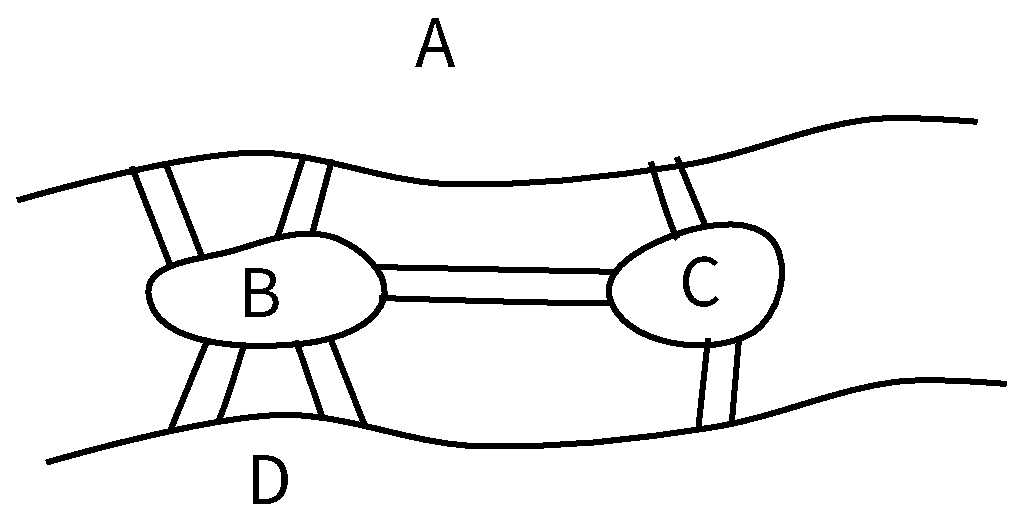
\includegraphics[width=5cm,height=4cm]{konigsberg} 
\end{frame}

\section{基本定义}
\begin{frame}
      \begin{thebibliography}{99}
  \bibitem[Sergey, 1997]{Sergey1997}Sergey Brin and Lawrence Page
\newblock   The Anatomy of a Large-Scale Hypertextual Web Search Engine.
\newblock WWW1997.
  \end{thebibliography}

\end{frame}
\begin{frame}
  \frametitle{6.2 基本定义}
设$V$为一个集合,$V$的一切二元子集之集合记为$\mathcal{P}_2(V)$,即
\begin{equation*}
  \mathcal{P}_2(V) = \{A|A \subseteq V \text{且} |A| = 2\}\text{。}
\end{equation*}
\begin{Def}\justifying\let\raggedright\justifying
  设$V$为一个非空有限集合,$E \subseteq \mathcal{P}_2(V)$,二元组$G = (V, E)$称为一个\alert{无向图}。$V$中的元素称为无向图$G$的\alert{顶点},$V$为\alert{顶点集};$E$中的元素称为无向图$G$的\alert{边},$E$为\alert{边集}。无向图简称\alert{图}。如果$|V|=p$,$|E|=q$,则称$G$为一个$(p,q)$图,即$G$为一个具有$p$个顶点$q$条边的图。
\end{Def}
      \centering
    \begin{tikzpicture}[auto,
    specification/.style ={circle, draw, thick, inner sep = 0pt, minimum size=2mm}]
   \node[specification] (A)  [label=0:$v_2$] at (18:1.3cm)  {};
   \node[specification] (B)  [label=90:$v_1$] at (90:1.3cm)  {};
   \node[specification] (C)  [label=180:$v_5$] at (162:1.3cm)  {};
   \node[specification] (D) [label=180:$v_4$] at (234:1.3cm)  {};
   \node[specification] (E)  [label=0:$v_3$] at (306:1.3cm)  {};      
   
   
   \draw[thick] (A) to  (B);
   \draw[thick] (B) to  (C);
   \draw[thick] (C) to  (D);
   \draw[thick] (D) to  (E);
   \draw[thick] (E) to  (A);
   \draw[thick] (A) to  (C);
   \draw[thick] (B) to  (E);
   \draw[thick] (C) to  (E);
   \draw[thick] (D) to  (A);
 \end{tikzpicture}
\end{frame}


\begin{frame}
  \frametitle{6.2 基本定义}
  \begin{Def}\justifying\let\raggedright\justifying
    在图$G=(V,E)$中,如果$\{u,v\}\in E$,则称\alert{顶点$u$与$v$邻接};若$x$与$y$为图$G$的两条边,并且仅有一个公共顶点,即$|x \cap y|= 1$,则称\alert{边$x$与$y$邻接};如果$x=\{u,v\}$为图$G$的一条边,则称\alert{$u$与$x$互相关联},同样的,称\alert{$v$与$x$互相关联}。
  \end{Def}
        \centering
    \begin{tikzpicture}[auto,
    specification/.style ={circle, draw, thick, inner sep = 0pt, minimum size=2mm}]
   \node[specification] (A)  [label=0:$v_2$] at (18:1.3cm)  {};
   \node[specification] (B)  [label=90:$v_1$] at (90:1.3cm)  {};
   \node[specification] (C)  [label=180:$v_5$] at (162:1.3cm)  {};
   \node[specification] (D) [label=180:$v_4$] at (234:1.3cm)  {};
   \node[specification] (E)  [label=0:$v_3$] at (306:1.3cm)  {};      
   
   
   \draw[thick] (A) to  (B);
   \draw[thick] (B) to  (C);
   \draw[thick] (C) to  (D);
   \draw[thick] (D) to  (E);
   \draw[thick] (E) to  (A);
   \draw[thick] (A) to  (C);
   \draw[thick] (B) to  (E);
   \draw[thick] (C) to  (E);
   \draw[thick] (D) to  (A);
 \end{tikzpicture}
\end{frame}

\begin{frame}
  \frametitle{6.2 基本定义}
  \begin{Def}
   如果一个图中两个顶点间允许有多于一条边存在,则称为\alert{多重图},这些边称为\alert{多重边}; 如果一个图中允许联结一个顶点与其自身的边存在,则称为\alert{带环图},这些边称为\alert{环};允许有环或多重边存在的图,称之为\alert{伪图}。
  \end{Def}
\end{frame}


\begin{frame}
  \frametitle{6.2 基本定义}
  \begin{Def}
设$G=(V,E)$为一个图,如果$E=\Phi$,则称$G$为\alert{零图}; $(1,0)$图称为\alert{平凡图}。    
  \end{Def}
\end{frame}



\begin{frame}
  \frametitle{6.2 基本定义}
  \begin{Def}
    设$v$为图$G=(V,E)$的任意一个顶点,$G$中与$v$关联的边的数目称为顶点$v$的\alert{度},记为$\deg v$。
  \end{Def}
   \centering
    \begin{tikzpicture}[auto,
    specification/.style ={circle, draw, thick, inner sep = 0pt, minimum size=2mm}]
   \node[specification] (A)  [label=0:$v_2$] at (18:1.3cm)  {};
   \node[specification] (B)  [label=90:$v_1$] at (90:1.3cm)  {};
   \node[specification] (C)  [label=180:$v_5$] at (162:1.3cm)  {};
   \node[specification] (D) [label=180:$v_4$] at (234:1.3cm)  {};
   \node[specification] (E)  [label=0:$v_3$] at (306:1.3cm)  {};      
   
   
   \draw[thick] (A) to  (B);
   \draw[thick] (B) to  (C);
   \draw[thick] (C) to  (D);
   \draw[thick] (D) to  (E);
   \draw[thick] (E) to  (A);
   \draw[thick] (A) to  (C);
   \draw[thick] (B) to  (E);
   \draw[thick] (C) to  (E);
   \draw[thick] (D) to  (A);
 \end{tikzpicture}
\\  G   
\end{frame}

\begin{frame}
  \frametitle{6.2 基本定义}
  \begin{Thm}
    设$G=(V,E)$为一个具有$p$个顶点$q$条边的图,则$G$中各顶点度的和等于边的条数$q$的两倍,即
        \begin{equation*}
      \sum_{v \in V}\deg v = 2q
    \end{equation*}
  \end{Thm}
    \centering
    \begin{tikzpicture}[auto,
    specification/.style ={circle, draw, thick, inner sep = 0pt, minimum size=2mm}]
   \node[specification] (A)  [label=0:$v_2$] at (18:1.3cm)  {};
   \node[specification] (B)  [label=90:$v_1$] at (90:1.3cm)  {};
   \node[specification] (C)  [label=180:$v_5$] at (162:1.3cm)  {};
   \node[specification] (D) [label=180:$v_4$] at (234:1.3cm)  {};
   \node[specification] (E)  [label=0:$v_3$] at (306:1.3cm)  {};      
   
   
   \draw[thick] (A) to  (B);
   \draw[thick] (B) to  (C);
   \draw[thick] (C) to  (D);
   \draw[thick] (D) to  (E);
   \draw[thick] (E) to  (A);
   \draw[thick] (A) to  (C);
   \draw[thick] (B) to  (E);
   \draw[thick] (C) to  (E);
   \draw[thick] (D) to  (A);
 \end{tikzpicture}
 \\  G   
\end{frame}


\begin{frame}
  \frametitle{6.2 基本定义}
  \begin{Thm}
       在任一图中,度为奇数的顶点的数目必为偶数。
  \end{Thm}
\centering
    \begin{tikzpicture}[auto,
    specification/.style ={circle, draw, thick, inner sep = 0pt, minimum size=2mm}]
   \node[specification] (A)  [label=0:$v_2$] at (18:1.3cm)  {};
   \node[specification] (B)  [label=90:$v_1$] at (90:1.3cm)  {};
   \node[specification] (C)  [label=180:$v_5$] at (162:1.3cm)  {};
   \node[specification] (D) [label=180:$v_4$] at (234:1.3cm)  {};
   \node[specification] (E)  [label=0:$v_3$] at (306:1.3cm)  {};      
   
   
   \draw[thick] (A) to  (B);
   \draw[thick] (B) to  (C);
   \draw[thick] (C) to  (D);
   \draw[thick] (D) to  (E);
   \draw[thick] (E) to  (A);
   \draw[thick] (A) to  (C);
   \draw[thick] (B) to  (E);
   \draw[thick] (C) to  (E);
   \draw[thick] (D) to  (A);
 \end{tikzpicture}
\\  G 
\end{frame}
\begin{frame}
  \frametitle{6.2 基本定义}
  \begin{Def}
    图$G$称为\alert{$r$度正则图},如果$G$的每个顶点的度都等于$r$。3度正则图也称为三次图。
    一个具有$p$个顶点的$p-1$度正则图称为包含$p$个顶点的\alert{完全图},记为$K_p$。
  \end{Def}
\end{frame}
\begin{frame}
  \frametitle{6.2 基本定义}
    \begin{minipage}[c]{0.4\textwidth}
\centering
    \begin{tikzpicture}[auto,
    specification/.style ={circle, draw, thick, inner sep = 0pt, minimum size=2mm}]
   \node[specification] (A)  [label=0:$v_2$] at (18:1.3cm)  {};
   \node[specification] (B)  [label=90:$v_1$] at (90:1.3cm)  {};
   \node[specification] (C)  [label=180:$v_5$] at (162:1.3cm)  {};
   \node[specification] (D) [label=180:$v_4$] at (234:1.3cm)  {};
   \node[specification] (E)  [label=0:$v_3$] at (306:1.3cm)  {};      
   
   
   \draw[thick] (A) to  (B);
   \draw[thick] (B) to  (C);
   \draw[thick] (C) to  (D);
   \draw[thick] (D) to  (E);
   \draw[thick] (E) to  (A);
   \draw[thick] (A) to  (C);
   \draw[thick] (B) to  (E);
   \draw[thick] (C) to  (E);
   \draw[thick] (D) to  (A);
 \end{tikzpicture}
\\ \centering G 
    \end{minipage}\hspace{2cm}
    \begin{minipage}[c]{0.4\textwidth}
\centering
    \begin{tikzpicture}[auto,
    specification/.style ={circle, draw, thick, inner sep = 0pt, minimum size=2mm}]
   \node[specification] (A)  [label=0:$v_2$] at (18:1.3cm)  {};
   \node[specification] (B)  [label=90:$v_1$] at (90:1.3cm)  {};
   \node[specification] (E)  [label=0:$v_3$] at (306:1.3cm)  {};      
   
   
   \draw[thick] (A) to  (B);
   \draw[thick] (B) to  (E);
 \end{tikzpicture}
\\ \centering H 
    \end{minipage}
    \pause
  \begin{Def}
    设$G=(V,E)$为一个图,图$H=(V_1,E_1)$称为$G$的一个子图,当且仅当$V_1$为$V$的
    非空子集且$E_1$为$E$的子集。如果$H \neq G$,则称$H$为$G$的\alert{真子图}。
  \end{Def}
\end{frame}

\begin{frame}
  \frametitle{6.2 基本定义}
  \begin{minipage}[c]{0.4\textwidth}
    \centering
    \begin{tikzpicture}[auto,
    specification/.style ={circle, draw, thick, inner sep = 0pt, minimum size=2mm}]
   \node[specification] (A)  [label=0:$v_2$] at (18:1.3cm)  {};
   \node[specification] (B)  [label=90:$v_1$] at (90:1.3cm)  {};
   \node[specification] (C)  [label=180:$v_5$] at (162:1.3cm)  {};
   \node[specification] (D) [label=180:$v_4$] at (234:1.3cm)  {};
   \node[specification] (E)  [label=0:$v_3$] at (306:1.3cm)  {};      
   
   
   \draw[thick] (A) to  (B);
   \draw[thick] (B) to  (C);
   \draw[thick] (C) to  (D);
   \draw[thick] (D) to  (E);
   \draw[thick] (E) to  (A);
   \draw[thick] (A) to  (C);
   \draw[thick] (B) to  (E);
   \draw[thick] (C) to  (E);
   \draw[thick] (D) to  (A);
 \end{tikzpicture}
\\ \centering G 
    \end{minipage}\hspace{2cm}
    \begin{minipage}[c]{0.4\textwidth}
\centering
    \begin{tikzpicture}[auto,
    specification/.style ={circle, draw, thick, inner sep = 0pt, minimum size=2mm}]
   \node[specification] (A)  [label=0:$v_2$] at (18:1.3cm)  {};
   \node[specification] (B)  [label=90:$v_1$] at (90:1.3cm)  {};
   \node[specification] (C)  [label=180:$v_5$] at (162:1.3cm)  {};
   \node[specification] (D) [label=180:$v_4$] at (234:1.3cm)  {};
   \node[specification] (E)  [label=0:$v_3$] at (306:1.3cm)  {};      
   
   
   \draw[thick] (A) to  (B);
   \draw[thick] (B) to  (E);
 \end{tikzpicture}
 \\ \centering H
    \end{minipage}
    \pause
  \begin{Def}
    设$G=(V,E)$为一个图,如果$F\subseteq E$,则称$G$的子图$H=(V,F)$ 为$G$的一个\alert{生成子图}。
  \end{Def}
\end{frame}

\begin{frame}
  \frametitle{6.2 基本定义}
    \begin{minipage}[c]{0.4\textwidth}
    \centering
    \begin{tikzpicture}[auto,
    specification/.style ={circle, draw, thick, inner sep = 0pt, minimum size=2mm}]
   \node[specification] (A)  [label=0:$v_2$] at (18:1.3cm)  {};
   \node[specification] (B)  [label=90:$v_1$] at (90:1.3cm)  {};
   \node[specification] (C)  [label=180:$v_5$] at (162:1.3cm)  {};
   \node[specification] (D) [label=180:$v_4$] at (234:1.3cm)  {};
   \node[specification] (E)  [label=0:$v_3$] at (306:1.3cm)  {};      
   
   
   \draw[thick] (A) to  (B);
   \draw[thick] (B) to  (C);
   \draw[thick] (C) to  (D);
   \draw[thick] (D) to  (E);
   \draw[thick] (E) to  (A);
   \draw[thick] (A) to  (C);
   \draw[thick] (B) to  (E);
   \draw[thick] (C) to  (E);
   \draw[thick] (D) to  (A);
 \end{tikzpicture}
 \\ \centering G 
    \end{minipage}\hspace{2cm}
    \begin{minipage}[c]{0.4\textwidth}
    \centering
    \begin{tikzpicture}[auto,
    specification/.style ={circle, draw, thick, inner sep = 0pt, minimum size=2mm}]
   \node[specification] (A)  [label=0:$v_2$] at (18:1.3cm)  {};
   \node[specification] (B)  [label=90:$v_1$] at (90:1.3cm)  {};
   \node[specification] (E)  [label=0:$v_3$] at (306:1.3cm)  {};      
   
   
   \draw[thick] (A) to  (B);
   \draw[thick] (E) to  (A);
   \draw[thick] (B) to  (E);
 \end{tikzpicture}
\\ \centering H 
    \end{minipage}

    \pause
  \begin{Def}
    设图$G$的子图$H$具有某种性质,若$G$中不存在与$H$不同的具有此性质且包含$H$的子图,则称$H$是具有此性质的\alert{极大子图}。
  \end{Def}
\pause
  \begin{Def}
    设$S$为图$G=(V,E)$的顶点集$V$的非空子集,则$G$的以$S$为顶点集的极大子图称为由$S$导出的子图,记为$\langle S \rangle$。
形式的,
\begin{equation*}
  \langle S \rangle=(S, \mathcal{P}_2(S) \cap E)
\end{equation*}
  \end{Def}
\end{frame}
\begin{frame}
  \frametitle{6.2 基本定义}
    \begin{minipage}[c]{0.4\textwidth}
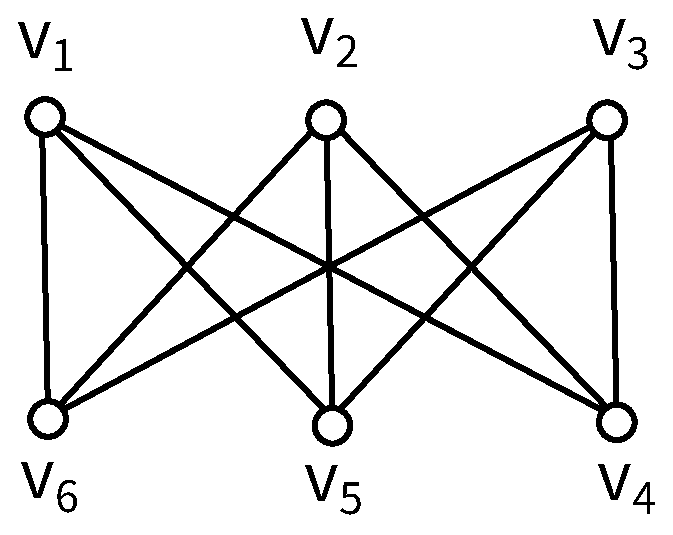
\includegraphics[width=4cm,height=3cm]{k33} \\ \centering G 
    \end{minipage}\hspace{2cm}
    \begin{minipage}[c]{0.4\textwidth}
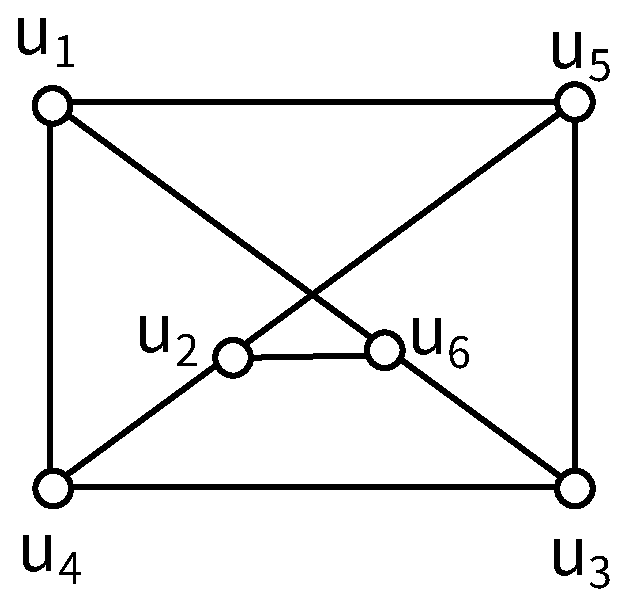
\includegraphics[width=4cm,height=3cm]{isomorphic} \\ \centering H 
    \end{minipage}
    \pause
  \begin{Def}
    设$G=(V,E)$, $H = (U, F)$为两个图,如果存在一个一一对应$\phi:V \to
    U$,使得$\{u,v\} \in E$当且仅当$\{\phi(u),\phi(v)\} \in F$,则称$G$与$H$\alert{同构}。
  \end{Def}
\end{frame}
\section{路、圈、连通图}
\begin{frame}[t]
  \begin{Exercise}
    判断:设具有6个顶点的图G和图G'各顶点的度都是依次为3,3,3,3,3,3,则G和G’同构。
  \end{Exercise}  
\end{frame}
\begin{frame}[t]
  \begin{Exercise}
    画出具有$4$个顶点的所有无向图(同构的只算一个)。
  \end{Exercise}  
\end{frame}
\begin{frame}
  \frametitle{6.3 路、圈、连通图}
  \begin{Def}
    设$G=(V,E)$为一个图。$G$的一条\alert{通道}是$G$的顶点和边的一个交错序列
    \[v_0,x_1,v_1,x_2,v_2,x_3,\ldots,v_{n-1},x_n,v_n\]
    其中$x_i=v_{i-1}v_i,i=1,2,\ldots,n$。$n$称为通道的长。这样的通道常称为$v_0-v_n$通道,并简记为$v_0v_1v_2\ldots   v_n$。当$v_0=v_n$时,则称此通道为\alert{闭通道}。
  \end{Def}
  \centering
  \begin{tikzpicture}[auto,
    specification/.style ={circle, draw, thick}]
   \node[specification] (E) [label=-135:$v_5$] at (0,0)  {};
   \node[specification] (F) [label=135:$v_3$] at (0,2)  {};
   \node[specification] (G) [label=45:$v_2$] at (2,2)  {};
   \node[specification] (H) [label=-45:$v_4$] at (2,0)  {};
   \node[specification] (I) [label=-45:$v_1$] at (4,2)  {};
   
   \draw[thick] (E) to  (F);
   \draw[thick] (F) to  (G);
   \draw[thick] (G) to  (H);
   \draw[thick] (H) to  (E);
   \draw[thick] (E) to  (G);
   \draw[thick] (G) to  (I);
   \draw[thick] (H) to  (I);
 \end{tikzpicture}  
 \\  G   
\end{frame}

\begin{frame}
  \frametitle{6.3 路、圈、连通图}
  \begin{Def}
   如果图中一条通道上的各边互不相同,则称此通道为图的\alert{迹}。如果一条闭通道上的各边互不相同,则称此闭通道为\alert{闭迹}。
  \end{Def}
  \centering
  \begin{tikzpicture}[auto,
    specification/.style ={circle, draw, thick}]
   \node[specification] (E) [label=-135:$v_5$] at (0,0)  {};
   \node[specification] (F) [label=135:$v_3$] at (0,2)  {};
   \node[specification] (G) [label=45:$v_2$] at (2,2)  {};
   \node[specification] (H) [label=-45:$v_4$] at (2,0)  {};
   \node[specification] (I) [label=-45:$v_1$] at (4,2)  {};
   
   \draw[thick] (E) to  (F);
   \draw[thick] (F) to  (G);
   \draw[thick] (G) to  (H);
   \draw[thick] (H) to  (E);
   \draw[thick] (E) to  (G);
   \draw[thick] (G) to  (I);
   \draw[thick] (H) to  (I);
 \end{tikzpicture}  
 \\  G   
\end{frame}

\begin{frame}
  \frametitle{6.3 路、圈、连通图}
  \begin{Def}
    如果一条通道上的各顶点互不相同,则称此通道为\alert{路}。如果一条长度大于$0$的闭迹上除终点外各顶点互不相同,则称此闭迹为\alert{圈},或\alert{回路}。
  \end{Def}
  \centering
  \begin{tikzpicture}[auto,
    specification/.style ={circle, draw, thick}]
   \node[specification] (E) [label=-135:$v_5$] at (0,0)  {};
   \node[specification] (F) [label=135:$v_3$] at (0,2)  {};
   \node[specification] (G) [label=45:$v_2$] at (2,2)  {};
   \node[specification] (H) [label=-45:$v_4$] at (2,0)  {};
   \node[specification] (I) [label=-45:$v_1$] at (4,2)  {};
   
   \draw[thick] (E) to  (F);
   \draw[thick] (F) to  (G);
   \draw[thick] (G) to  (H);
   \draw[thick] (H) to  (E);
   \draw[thick] (E) to  (G);
   \draw[thick] (G) to  (I);
   \draw[thick] (H) to  (I);
 \end{tikzpicture}  
 \\  G   
\end{frame}

\begin{frame}
  \frametitle{6.3 路、圈、连通图}
  \begin{Def}
   设$G=(V,E)$为一个图,如果$G$中任两个不同顶点间至少有一条路联结,则称$G$为一个\alert{连通图}。
  \end{Def}
    \centering
    \begin{tikzpicture}[auto,
    specification/.style ={circle, draw, thick, inner sep = 0pt, minimum size=2mm}]
   \node[specification] (A)  [label=0:$v_2$] at (18:1.3cm)  {};
   \node[specification] (B)  [label=90:$v_1$] at (90:1.3cm)  {};
   \node[specification] (C)  [label=180:$v_5$] at (162:1.3cm)  {};
   \node[specification] (D) [label=180:$v_4$] at (234:1.3cm)  {};
   \node[specification] (E)  [label=0:$v_3$] at (306:1.3cm)  {};      
   
   
   \draw[thick] (A) to  (B);
   \draw[thick] (B) to  (C);
   \draw[thick] (C) to  (D);
   \draw[thick] (D) to  (E);
   \draw[thick] (E) to  (A);
   \draw[thick] (A) to  (C);
   \draw[thick] (B) to  (E);
   \draw[thick] (C) to  (E);
   \draw[thick] (D) to  (A);
 \end{tikzpicture}
 \\  G   
\end{frame}

\begin{frame}
  \frametitle{6.3 路、圈、连通图}
  \centering
  \begin{minipage}{0.33\linewidth}
    \centering
    \begin{tikzpicture}[auto,
    specification/.style ={circle, draw, thick}]
   \node[specification] (A) [label=-135:$v_1$] at (0,0)  {};
   \node[specification] (B) [label=135:$v_2$] at (0,2)  {};
   \node[specification] (C) [label=45:$v_3$] at (2,2)  {};
   \node[specification] (D) [label=-45:$v_4$] at (2,0)  {};
   \draw[thick] (A) to  (B);
   \draw[thick] (B) to  (C);
   \draw[thick] (C) to  (D);
   \draw[thick] (D) to  (A);
 \end{tikzpicture}
\end{minipage}\hfill
\begin{minipage}{0.33\linewidth}
  \centering
  \begin{tikzpicture}[auto,
    specification/.style ={circle, draw, thick}]
   \node[specification] (E) [label=-135:$v_5$] at (0,0)  {};
   \node[specification] (F) [label=135:$v_6$] at (0,2)  {};
   \node[specification] (G) [label=45:$v_7$] at (2,2)  {};
   \node[specification] (H) [label=-45:$v_8$] at (2,0)  {};
   \draw[thick] (E) to  (F);
   \draw[thick] (F) to  (G);
   \draw[thick] (G) to  (H);
   \draw[thick] (H) to  (E);
   \draw[thick] (E) to  (G);
 \end{tikzpicture}  
\end{minipage}\hfill
\begin{minipage}{0.33\linewidth}
  \centering
  \begin{tikzpicture}[auto,
    specification/.style ={circle, draw, thick}]
   \node[specification] (I) [label=-135:$v_9$] at (0,0)  {};
   \node[specification] (J) [label=135:$v_{10}$] at (1,2)  {};
   \node[specification] (K) [label=-45:$v_{11}$] at (2,0)  {};
   \draw[thick] (I) to  (J);
   \draw[thick] (J) to  (K);
 \end{tikzpicture}
\end{minipage}
\vspace*{2cm}
$G$
\end{frame}

% \begin{frame}
%   \frametitle{6.3 路、圈、连通图}
%   \begin{minipage}{0.33\linewidth}
%     \centering
%     \begin{tikzpicture}[auto,
%     specification/.style ={circle, draw, thick}]
%    \node[specification] (A) [label=-135:$v_1$] at (0,0)  {};
%    \node[specification] (B) [label=135:$v_2$] at (0,2)  {};
%    \node[specification] (C) [label=45:$v_3$] at (2,2)  {};
%    \node[specification] (D) [label=-45:$v_4$] at (2,0)  {};
%    \draw[thick] (A) to  (B);
%    \draw[thick] (B) to  (C);
%    \draw[thick] (C) to  (D);
%    \draw[thick] (D) to  (A);
%  \end{tikzpicture}\\
%  $G_1$
% \end{minipage}\hfill
% \begin{minipage}{0.33\linewidth}
%   \centering
%   \begin{tikzpicture}[auto,
%     specification/.style ={circle, draw, thick}]
%    \node[specification] (E) [label=-135:$v_5$] at (0,0)  {};
%    \node[specification] (F) [label=135:$v_6$] at (0,2)  {};
%    \node[specification] (G) [label=45:$v_7$] at (2,2)  {};
%    \node[specification] (H) [label=-45:$v_8$] at (2,0)  {};
%    \draw[thick] (E) to  (F);
%    \draw[thick] (F) to  (G);
%    \draw[thick] (G) to  (H);
%    \draw[thick] (H) to  (E);
%    \draw[thick] (E) to  (G);
%  \end{tikzpicture}  \\
%  $G_2$
% \end{minipage}\hfill
% \begin{minipage}{0.33\linewidth}
%   \centering
%   \begin{tikzpicture}[auto,
%     specification/.style ={circle, draw, thick}]
%    \node[specification] (I) [label=-135:$v_9$] at (0,0)  {};
%    \node[specification] (J) [label=135:$v_{10}$] at (1,2)  {};
%    \node[specification] (K) [label=-45:$v_{11}$] at (2,0)  {};
%    \draw[thick] (I) to  (J);
%    \draw[thick] (J) to  (K);
%  \end{tikzpicture}\\
%  $G_3$
% \end{minipage}
% \end{frame}
\begin{frame}
    \centering
  \begin{minipage}{0.24\linewidth}
    \centering
    \begin{tikzpicture}[auto,
    specification/.style ={circle, draw, thick}]
   \node[specification] (A) at (0,0)  {};
   \node[specification] (B)  at (0,1)  {};
   \node[specification] (C)  at (1,1)  {};
   \node[specification] (D) at (1,0)  {};
 \end{tikzpicture}\\
 \vspace*{0.1cm}
 A
\end{minipage}\hfill 
  \begin{minipage}{0.24\linewidth}
    \centering
    \begin{tikzpicture}[auto,
    specification/.style ={circle, draw, thick}]
   \node[specification] (A) at (0,0)  {};
   \node[specification] (B) at (0,1)  {};
   \node[specification] (C) at (1,1)  {};
   \node[specification] (D) at (1,0)  {};
   \draw[thick] (B) to  (C);
 \end{tikzpicture}\\
 \vspace*{0.1cm}
 B
\end{minipage}\hfill 
  \begin{minipage}{0.24\linewidth}
    \centering
    \begin{tikzpicture}[auto,
    specification/.style ={circle, draw, thick}]
   \node[specification] (A) at (0,0)  {};
   \node[specification] (B) at (0,1)  {};
   \node[specification] (C) at (1,1)  {};
   \node[specification] (D) at (1,0)  {};
   \draw[thick] (A) to  (B);
   \draw[thick] (B) to  (C);
 \end{tikzpicture}\\
 \vspace*{0.1cm}
 C
\end{minipage}\hfill 
  \begin{minipage}{0.24\linewidth}
    \centering
    \begin{tikzpicture}[auto,
    specification/.style ={circle, draw, thick}]
   \node[specification] (A)  at (0,0)  {};
   \node[specification] (B)  at (0,1)  {};
   \node[specification] (C)  at (1,1)  {};
   \node[specification] (D) at (1,0)  {};
   \draw[thick] (B) to  (C);
   \draw[thick] (D) to  (A);
 \end{tikzpicture}\\
 \vspace*{0.1cm}
 D
\end{minipage}\hfill

\vspace*{0.5cm}
  \begin{minipage}{0.24\linewidth}
    \centering
    \begin{tikzpicture}[auto,
    specification/.style ={circle, draw, thick}]
   \node[specification] (A) at (0,0)  {};
   \node[specification] (B)  at (0,1)  {};
   \node[specification] (C)  at (1,1)  {};
   \node[specification] (D) at (1,0)  {};
   \draw[thick] (A) to (B);
   \draw[thick] (B) to (C);
      \draw[thick] (B) to (D);
 \end{tikzpicture}\\
 \vspace*{0.1cm}
 E
\end{minipage}\hfill
  \begin{minipage}{0.24\linewidth}
    \centering
    \begin{tikzpicture}[auto,
    specification/.style ={circle, draw, thick}]
   \node[specification] (A) at (0,0)  {};
   \node[specification] (B) at (0,1)  {};
   \node[specification] (C) at (1,1)  {};
   \node[specification] (D) at (1,0)  {};
   \draw[thick] (A) to  (B);
   \draw[thick] (B) to (C);
   \draw[thick] (C) to (A);
 \end{tikzpicture}\\
 \vspace*{0.1cm}
 F
\end{minipage}\hfill
  \begin{minipage}{0.24\linewidth}
    \centering
    \begin{tikzpicture}[auto,
    specification/.style ={circle, draw, thick}]
   \node[specification] (A) at (0,0)  {};
   \node[specification] (B) at (0,1)  {};
   \node[specification] (C) at (1,1)  {};
   \node[specification] (D) at (1,0)  {};
   \draw[thick] (A) to  (B);
   \draw[thick] (B) to  (C);
      \draw[thick] (C) to (D);
 \end{tikzpicture}\\
 \vspace*{0.1cm}
 G
\end{minipage}\hfill 
  \begin{minipage}{0.24\linewidth}
    \centering
    \begin{tikzpicture}[auto,
    specification/.style ={circle, draw, thick}]
   \node[specification] (A)   at (0,0)  {};
   \node[specification] (B)  at (0,1)  {};
   \node[specification] (C)  at (1,1)  {};
   \node[specification] (D) at (1,0)  {};
   \draw[thick] (A) to  (C);
   \draw[thick] (C) to  (D);
   \draw[thick] (D) to (A);
   \draw[thick] (B) to (D);
 \end{tikzpicture}\\
 \vspace*{0.1cm}
 H
\end{minipage}\hfill 

\vspace*{0.5cm}
\flushleft
  \begin{minipage}{0.24\linewidth}
    \centering
    \begin{tikzpicture}[auto,
    specification/.style ={circle, draw, thick}]
   \node[specification] (A) at (0,0)  {};
   \node[specification] (B)  at (0,1)  {};
   \node[specification] (C)  at (1,1)  {};
   \node[specification] (D) at (1,0)  {};
   \draw[thick] (A) to (B);
   \draw[thick] (B) to (D);
   \draw[thick] (D) to (C);
      \draw[thick] (C) to (A);
 \end{tikzpicture}\\
 \vspace*{0.1cm}
 I
\end{minipage}
  \begin{minipage}{0.24\linewidth}
    \centering
    \begin{tikzpicture}[auto,
    specification/.style ={circle, draw, thick}]
   \node[specification] (A) at (0,0)  {};
   \node[specification] (B) at (0,1)  {};
   \node[specification] (C) at (1,1)  {};
   \node[specification] (D) at (1,0)  {};
   \draw[thick] (A) to  (B);
      \draw[thick] (C) to (D);
   \draw[thick] (D) to (A);
   \draw[thick] (A) to (C);
   \draw[thick] (B) to (D);
 \end{tikzpicture}\\
 \vspace*{0.1cm}
 J
\end{minipage} 
  \begin{minipage}{0.24\linewidth}
    \centering
    \begin{tikzpicture}[auto,
    specification/.style ={circle, draw, thick}]
   \node[specification] (A) at (0,0)  {};
   \node[specification] (B) at (0,1)  {};
   \node[specification] (C) at (1,1)  {};
   \node[specification] (D) at (1,0)  {};
   \draw[thick] (A) to  (B);
   \draw[thick] (B) to  (C);
      \draw[thick] (C) to (D);
   \draw[thick] (D) to (A);
   \draw[thick] (A) to (C);
   \draw[thick] (B) to (D);
 \end{tikzpicture}\\
 \vspace*{0.1cm}
 K
\end{minipage}  
\end{frame}

\begin{frame}
  \frametitle{6.3 路、圈、连通图}
  \begin{Def}
    图$G$的极大连通子图称为$G$的一个\alert{支}。
  \end{Def}
    \centering
  \begin{minipage}{0.33\linewidth}
    \centering
    \begin{tikzpicture}[auto,
    specification/.style ={circle, draw, thick}]
   \node[specification] (A) [label=-135:$v_1$] at (0,0)  {};
   \node[specification] (B) [label=135:$v_2$] at (0,2)  {};
   \node[specification] (C) [label=45:$v_3$] at (2,2)  {};
   \node[specification] (D) [label=-45:$v_4$] at (2,0)  {};
   \draw[thick] (A) to  (B);
   \draw[thick] (B) to  (C);
   \draw[thick] (C) to  (D);
   \draw[thick] (D) to  (A);
 \end{tikzpicture}
\end{minipage}\hfill
\begin{minipage}{0.33\linewidth}
  \centering
  \begin{tikzpicture}[auto,
    specification/.style ={circle, draw, thick}]
   \node[specification] (E) [label=-135:$v_5$] at (0,0)  {};
   \node[specification] (F) [label=135:$v_6$] at (0,2)  {};
   \node[specification] (G) [label=45:$v_7$] at (2,2)  {};
   \node[specification] (H) [label=-45:$v_8$] at (2,0)  {};
   \draw[thick] (E) to  (F);
   \draw[thick] (F) to  (G);
   \draw[thick] (G) to  (H);
   \draw[thick] (H) to  (E);
   \draw[thick] (E) to  (G);
 \end{tikzpicture}  
\end{minipage}\hfill
\begin{minipage}{0.33\linewidth}
  \centering
  \begin{tikzpicture}[auto,
    specification/.style ={circle, draw, thick}]
   \node[specification] (I) [label=-135:$v_9$] at (0,0)  {};
   \node[specification] (J) [label=135:$v_{10}$] at (1,2)  {};
   \node[specification] (K) [label=-45:$v_{11}$] at (2,0)  {};
   \draw[thick] (I) to  (J);
   \draw[thick] (J) to  (K);
 \end{tikzpicture}
\end{minipage}
\vspace*{2cm}
$G$

\end{frame}

\begin{frame}
  \frametitle{6.3 路、圈、连通图}
  \begin{Thm}
    设$G=(V,E)$是一个图。在$V$上定义二元关系$\cong$如下:\[\forall u, v \in V, u
      \cong v\text{当且仅当}u\text{与}v\text{间有一条路,}\]则$\cong$为$V$上的等价关系,$G$的支就是关于$\cong$的每个等价类的导出子图。
  \end{Thm}

      \centering
  \begin{minipage}{0.33\linewidth}
    \centering
    \begin{tikzpicture}[auto,
    specification/.style ={circle, draw, thick}]
   \node[specification] (A) [label=-135:$v_1$] at (0,0)  {};
   \node[specification] (B) [label=135:$v_2$] at (0,2)  {};
   \node[specification] (C) [label=45:$v_3$] at (2,2)  {};
   \node[specification] (D) [label=-45:$v_4$] at (2,0)  {};
   \draw[thick] (A) to  (B);
   \draw[thick] (B) to  (C);
   \draw[thick] (C) to  (D);
   \draw[thick] (D) to  (A);
 \end{tikzpicture}
\end{minipage}\hfill
\begin{minipage}{0.33\linewidth}
  \centering
  \begin{tikzpicture}[auto,
    specification/.style ={circle, draw, thick}]
   \node[specification] (E) [label=-135:$v_5$] at (0,0)  {};
   \node[specification] (F) [label=135:$v_6$] at (0,2)  {};
   \node[specification] (G) [label=45:$v_7$] at (2,2)  {};
   \node[specification] (H) [label=-45:$v_8$] at (2,0)  {};
   \draw[thick] (E) to  (F);
   \draw[thick] (F) to  (G);
   \draw[thick] (G) to  (H);
   \draw[thick] (H) to  (E);
   \draw[thick] (E) to  (G);
 \end{tikzpicture}  
\end{minipage}\hfill
\begin{minipage}{0.33\linewidth}
  \centering
  \begin{tikzpicture}[auto,
    specification/.style ={circle, draw, thick}]
   \node[specification] (I) [label=-135:$v_9$] at (0,0)  {};
   \node[specification] (J) [label=135:$v_{10}$] at (1,2)  {};
   \node[specification] (K) [label=-45:$v_{11}$] at (2,0)  {};
   \draw[thick] (I) to  (J);
   \draw[thick] (J) to  (K);
 \end{tikzpicture}
\end{minipage}
\vspace*{2cm}
$G$



\end{frame}


\section{补图、偶图}
\begin{frame}
  \frametitle{6.4 补图、偶图}
  \begin{Def}
    设$G=(V,E)$是一个图,图$G^c=(V, \mathcal{P}_2(V)\setminus E)$称为$G$的\alert{补图}。
  \end{Def}
\end{frame}

\begin{frame}
    \centering
  \begin{minipage}{0.24\linewidth}
    \centering
    \begin{tikzpicture}[auto,
    specification/.style ={circle, draw, thick}]
   \node[specification] (A) at (0,0)  {};
   \node[specification] (B)  at (0,1)  {};
   \node[specification] (C)  at (1,1)  {};
   \node[specification] (D) at (1,0)  {};
 \end{tikzpicture}\\
 \vspace*{0.1cm}
 A
\end{minipage}\hfill 
  \begin{minipage}{0.24\linewidth}
    \centering
    \begin{tikzpicture}[auto,
    specification/.style ={circle, draw, thick}]
   \node[specification] (A) at (0,0)  {};
   \node[specification] (B) at (0,1)  {};
   \node[specification] (C) at (1,1)  {};
   \node[specification] (D) at (1,0)  {};
   \draw[thick] (B) to  (C);
 \end{tikzpicture}\\
 \vspace*{0.1cm}
 B
\end{minipage}\hfill 
  \begin{minipage}{0.24\linewidth}
    \centering
    \begin{tikzpicture}[auto,
    specification/.style ={circle, draw, thick}]
   \node[specification] (A) at (0,0)  {};
   \node[specification] (B) at (0,1)  {};
   \node[specification] (C) at (1,1)  {};
   \node[specification] (D) at (1,0)  {};
   \draw[thick] (A) to  (B);
   \draw[thick] (B) to  (C);
 \end{tikzpicture}\\
 \vspace*{0.1cm}
 C
\end{minipage}\hfill 
  \begin{minipage}{0.24\linewidth}
    \centering
    \begin{tikzpicture}[auto,
    specification/.style ={circle, draw, thick}]
   \node[specification] (A)  at (0,0)  {};
   \node[specification] (B)  at (0,1)  {};
   \node[specification] (C)  at (1,1)  {};
   \node[specification] (D) at (1,0)  {};
   \draw[thick] (B) to  (C);
   \draw[thick] (D) to  (A);
 \end{tikzpicture}\\
 \vspace*{0.1cm}
 D
\end{minipage}\hfill

\vspace*{0.5cm}
  \begin{minipage}{0.24\linewidth}
    \centering
    \begin{tikzpicture}[auto,
    specification/.style ={circle, draw, thick}]
   \node[specification] (A) at (0,0)  {};
   \node[specification] (B)  at (0,1)  {};
   \node[specification] (C)  at (1,1)  {};
   \node[specification] (D) at (1,0)  {};
   \draw[thick] (A) to (B);
   \draw[thick] (B) to (C);
      \draw[thick] (B) to (D);
 \end{tikzpicture}\\
 \vspace*{0.1cm}
 E
\end{minipage}\hfill
  \begin{minipage}{0.24\linewidth}
    \centering
    \begin{tikzpicture}[auto,
    specification/.style ={circle, draw, thick}]
   \node[specification] (A) at (0,0)  {};
   \node[specification] (B) at (0,1)  {};
   \node[specification] (C) at (1,1)  {};
   \node[specification] (D) at (1,0)  {};
   \draw[thick] (A) to  (C);
   \draw[thick] (C) to (D);
      \draw[thick] (D) to (A);
 \end{tikzpicture}\\
 \vspace*{0.1cm}
 F
\end{minipage}\hfill
  \begin{minipage}{0.24\linewidth}
    \centering
    \begin{tikzpicture}[auto,
    specification/.style ={circle, draw, thick}]
   \node[specification] (A) at (0,0)  {};
   \node[specification] (B) at (0,1)  {};
   \node[specification] (C) at (1,1)  {};
   \node[specification] (D) at (1,0)  {};
   \draw[thick] (A) to  (B);
   \draw[thick] (B) to  (C);
      \draw[thick] (C) to (D);
 \end{tikzpicture}\\
 \vspace*{0.1cm}
 G
\end{minipage}\hfill 
  \begin{minipage}{0.24\linewidth}
    \centering
    \begin{tikzpicture}[auto,
    specification/.style ={circle, draw, thick}]
   \node[specification] (A)  at (0,0)  {};
   \node[specification] (B)  at (0,1)  {};
   \node[specification] (C)  at (1,1)  {};
   \node[specification] (D) at (1,0)  {};
   \draw[thick] (A) to  (C);
   \draw[thick] (C) to  (D);
   \draw[thick] (D) to (A);
   \draw[thick] (B) to (D);
 \end{tikzpicture}\\
 \vspace*{0.1cm}
 H
\end{minipage}\hfill 

\vspace*{0.5cm}
\flushleft
  \begin{minipage}{0.24\linewidth}
    \centering
    \begin{tikzpicture}[auto,
    specification/.style ={circle, draw, thick}]
   \node[specification] (A) at (0,0)  {};
   \node[specification] (B)  at (0,1)  {};
   \node[specification] (C)  at (1,1)  {};
   \node[specification] (D) at (1,0)  {};
   \draw[thick] (A) to (B);
   \draw[thick] (B) to (D);
   \draw[thick] (D) to (C);
      \draw[thick] (C) to (A);
 \end{tikzpicture}\\
 \vspace*{0.1cm}
 I
\end{minipage}
  \begin{minipage}{0.24\linewidth}
    \centering
    \begin{tikzpicture}[auto,
    specification/.style ={circle, draw, thick}]
   \node[specification] (A) at (0,0)  {};
   \node[specification] (B) at (0,1)  {};
   \node[specification] (C) at (1,1)  {};
   \node[specification] (D) at (1,0)  {};
   \draw[thick] (A) to  (B);
      \draw[thick] (C) to (D);
   \draw[thick] (D) to (A);
   \draw[thick] (A) to (C);
   \draw[thick] (B) to (D);
 \end{tikzpicture}\\
 \vspace*{0.1cm}
 J
\end{minipage} 
  \begin{minipage}{0.24\linewidth}
    \centering
    \begin{tikzpicture}[auto,
    specification/.style ={circle, draw, thick}]
   \node[specification] (A) at (0,0)  {};
   \node[specification] (B) at (0,1)  {};
   \node[specification] (C) at (1,1)  {};
   \node[specification] (D) at (1,0)  {};
   \draw[thick] (A) to  (B);
   \draw[thick] (B) to  (C);
      \draw[thick] (C) to (D);
   \draw[thick] (D) to (A);
   \draw[thick] (A) to (C);
   \draw[thick] (B) to (D);
 \end{tikzpicture}\\
 \vspace*{0.1cm}
 K
\end{minipage}  
\end{frame}
\begin{frame}
  \frametitle{6.4 补图、偶图}
  \begin{Def}
   如果$G$与$G^c$同构,则称$G$为\alert{自补图}。
  \end{Def}
\end{frame}

\begin{frame}
  \frametitle{6.4 补图、偶图}
  \begin{Thm}
    对任一有$6$个顶点的图$G$,$G$中或$G^c$中有一个三角形。
  \end{Thm}
  \begin{proof}[证明]
    设图$G$的顶点集为$V=\{v_1,v_2,v_3,v_4,v_5,v_6\}$,考虑顶点$v_1$。
    \begin{itemize}
    \item 存在三个顶点,其中的每个顶点都与顶点$v_1$相邻接。不失一般性,不妨设这
      个三个顶点为$v_2,v_3,v_4$。
      \begin{itemize}
      \item[-] 在顶点$v_2,v_3,v_4$中,存在两个顶点相邻接,此时$G$中存在三角形。
      \item[-] 在顶点$v_2,v_3,v_4$中,任意两个顶点都不邻接,此时$G^c$中存在三角形。
      \end{itemize}
    \item 存在三个顶点,其中的每个顶点都与顶点$v_1$不邻接。不失一般性,不妨设这
      个三个顶点为$v_2,v_3,v_4$。
      \begin{itemize}
      \item[-] 在顶点$v_2,v_3,v_4$中,存在两个顶点不邻接,此时$G^c$中存在三角形。
      \item[-] 在顶点$v_2,v_3,v_4$中,任意两个顶点互相邻接,此时$G$中存在三角形。
      \end{itemize}

    \end{itemize}
  \end{proof}
\end{frame}

% \begin{frame}
%   \frametitle{6.4 补图、偶图}
%   \begin{Def}
%     对任意的正整数$m$,$n$,$m \geq 2$,$n \geq 2$,求一个最小的正整数$r(m,n)$,
%     使得任何有$r(m,n)$个顶点的图$G$中一定含有一个$K_m$或者图$G^c$中一定含有一个$K_n$,这里的数$r(m,n)$称为\alert{拉姆齐数}。
%   \end{Def}
% \end{frame}

\begin{frame}
  \frametitle{6.4 补图、偶图}
  \begin{Def}\justifying\let\raggedright\justifying
    设$G=(V,E)$为一个图,如果$G$的顶点集$V$有一个二划分$\{V_1,V_2\}$,
    使得$G$的任一条边的两个端点一个在$V_1$中,另一个在$V_2$中,则称$G$为\alert{偶图}。如果$\forall u \in V_1, v \in V_2$均有$uv \in E$,则称$G$为\alert{完全偶图},记为$K_{m,n}$,其中$|V_1|=m,|V_2|=n$。
  \end{Def}
\end{frame}

\begin{frame}
  \frametitle{6.4 补图、偶图}
  \begin{Def}
    设$G=(V,E)$是一个图,$u$和$v$是$G$的顶点。联结$u$和$v$的最短路的长称为$u$与$v$之间的\alert{距离},并记为$d(u,v)$。如果$u$与$v$间在$G$中没有路,则定义$d(u,v)=\infty$。
  \end{Def}
\end{frame}

\begin{frame}
  \frametitle{6.4 补图、偶图}
  \begin{Thm}
    图$G$为偶图的充分必要条件为它的所有圈都是偶数长。
  \end{Thm}
  A graph is bipartite if and only if it contains no cycles with odd lengths.
  
  \pause
  Proof.


  \pause
    Suppose that G is bipartite with bipartition (X, Y), \pause and let $C=v_0v_1\ldots v_kv_0$ be a cycle of G.
   \pause Without loss of generality we may assume that $v_0\in X$. \pause Then, \pause since $v_0v_1\in E$ and G is bipartite, 
   \pause  $v_1\in Y$. \pause In general, \pause $v_{2i}\in X$ and $v_{2i+1}\in Y$.\pause Since $v_0\in X$, \pause $v_k\in Y$. \pause Thus $k=2i+1$, for some $i$, \pause and it follows that $C$ is even.

\end{frame}
\begin{frame}
  \pause It clearly suffices to prove the converse for connected graphs.\pause Let $G$ be a
    connected graph that contains no odd cycles.\pause We choose an arbitrary vertex $u$ 
    and define a partition (X, Y) of V by setting
    \begin{align*}
      X&=\{x\in V | d(u,x) \text{is even}\}\\
      Y&=\{y\in V| d(u,y) \text{is odd}\}
    \end{align*}
   \pause We shall show that (X, Y) is a bipartition of G. \pause Suppose that $v$ and $w$ are
    two vertices of X. \pause Let P be a shortest (u,v)-path and Q be a shortest (u,w)-path.
   \pause Denote by $u_1$ the last vertex common to P and Q. \pause Since P and Q are shortest paths, 
  \pause  the $(u,u_1)$-sections of both P and Q are shortest $(u,u_1)$-paths and, \pause therefore, \pause have
    the same length. \pause Now, \pause since the lengths of both P and Q are even,\pause the lengths of the $(u_1,v)$-section
    $P_1$ of P and the $(u_1,w)$-section $Q_1$ of Q must have the same parity. \pause It follows that the $(v,w)$-path from $v$ to $u_1$ along $P_1$ reversely and then from $u_1$ to $w$ along $Q_1$
    is of even length. \pause If $v$ were joined to w, \pause the path from $v$ to $u_1$ along $P_1$ reversely,\pause from $u_1$ to $w$ along $Q_1$ and then from $w$ to $v$ along the edge $wv$ would be a cycle of odd length, \pause contrary to the hypothesis. \pause Therefore no
    two vertices in X are adjacent; \pause similarly, \pause no two vertices in Y are adjacent.
\end{frame}

\begin{frame}
    \centering
  \begin{minipage}{0.24\linewidth}
    \centering
    \begin{tikzpicture}[auto,
    specification/.style ={circle, draw, thick}]
   \node[specification] (A) at (0,0)  {};
   \node[specification] (B)  at (0,1)  {};
   \node[specification] (C)  at (1,1)  {};
   \node[specification] (D) at (1,0)  {};
 \end{tikzpicture}\\
 \vspace*{0.1cm}
 A
\end{minipage}\hfill 
  \begin{minipage}{0.24\linewidth}
    \centering
    \begin{tikzpicture}[auto,
    specification/.style ={circle, draw, thick}]
   \node[specification] (A) at (0,0)  {};
   \node[specification] (B) at (0,1)  {};
   \node[specification] (C) at (1,1)  {};
   \node[specification] (D) at (1,0)  {};
   \draw[thick] (B) to  (C);
 \end{tikzpicture}\\
 \vspace*{0.1cm}
 B
\end{minipage}\hfill 
  \begin{minipage}{0.24\linewidth}
    \centering
    \begin{tikzpicture}[auto,
    specification/.style ={circle, draw, thick}]
   \node[specification] (A) at (0,0)  {};
   \node[specification] (B) at (0,1)  {};
   \node[specification] (C) at (1,1)  {};
   \node[specification] (D) at (1,0)  {};
   \draw[thick] (A) to  (B);
   \draw[thick] (B) to  (C);
 \end{tikzpicture}\\
 \vspace*{0.1cm}
 C
\end{minipage}\hfill 
  \begin{minipage}{0.24\linewidth}
    \centering
    \begin{tikzpicture}[auto,
    specification/.style ={circle, draw, thick}]
   \node[specification] (A)  at (0,0)  {};
   \node[specification] (B)  at (0,1)  {};
   \node[specification] (C)  at (1,1)  {};
   \node[specification] (D) at (1,0)  {};
   \draw[thick] (B) to  (C);
   \draw[thick] (D) to  (A);
 \end{tikzpicture}\\
 \vspace*{0.1cm}
 D
\end{minipage}\hfill

\vspace*{0.5cm}
  \begin{minipage}{0.24\linewidth}
    \centering
    \begin{tikzpicture}[auto,
    specification/.style ={circle, draw, thick}]
   \node[specification] (A) at (0,0)  {};
   \node[specification] (B)  at (0,1)  {};
   \node[specification] (C)  at (1,1)  {};
   \node[specification] (D) at (1,0)  {};
   \draw[thick] (A) to (B);
   \draw[thick] (B) to (C);
      \draw[thick] (B) to (D);
 \end{tikzpicture}\\
 \vspace*{0.1cm}
 E
\end{minipage}\hfill
  \begin{minipage}{0.24\linewidth}
    \centering
    \begin{tikzpicture}[auto,
    specification/.style ={circle, draw, thick}]
   \node[specification] (A) at (0,0)  {};
   \node[specification] (B) at (0,1)  {};
   \node[specification] (C) at (1,1)  {};
   \node[specification] (D) at (1,0)  {};
   \draw[thick] (A) to  (B);
   \draw[thick] (B) to (C);
   \draw[thick] (C) to (A);
 \end{tikzpicture}\\
 \vspace*{0.1cm}
 F
\end{minipage}\hfill
  \begin{minipage}{0.24\linewidth}
    \centering
    \begin{tikzpicture}[auto,
    specification/.style ={circle, draw, thick}]
   \node[specification] (A) at (0,0)  {};
   \node[specification] (B) at (0,1)  {};
   \node[specification] (C) at (1,1)  {};
   \node[specification] (D) at (1,0)  {};
   \draw[thick] (A) to  (B);
   \draw[thick] (B) to  (C);
      \draw[thick] (C) to (D);
 \end{tikzpicture}\\
 \vspace*{0.1cm}
 G
\end{minipage}\hfill 
  \begin{minipage}{0.24\linewidth}
    \centering
    \begin{tikzpicture}[auto,
    specification/.style ={circle, draw, thick}]
   \node[specification] (A)  at (0,0)  {};
   \node[specification] (B)  at (0,1)  {};
   \node[specification] (C)  at (1,1)  {};
   \node[specification] (D) at (1,0)  {};
   \draw[thick] (A) to  (C);
   \draw[thick] (C) to  (D);
   \draw[thick] (D) to (A);
   \draw[thick] (B) to (D);
 \end{tikzpicture}\\
 \vspace*{0.1cm}
 H
\end{minipage}\hfill 

\vspace*{0.5cm}
\flushleft
  \begin{minipage}{0.24\linewidth}
    \centering
    \begin{tikzpicture}[auto,
    specification/.style ={circle, draw, thick}]
   \node[specification] (A) at (0,0)  {};
   \node[specification] (B)  at (0,1)  {};
   \node[specification] (C)  at (1,1)  {};
   \node[specification] (D) at (1,0)  {};
   \draw[thick] (A) to (B);
   \draw[thick] (B) to (D);
   \draw[thick] (D) to (C);
      \draw[thick] (C) to (A);
 \end{tikzpicture}\\
 \vspace*{0.1cm}
 I
\end{minipage}
  \begin{minipage}{0.24\linewidth}
    \centering
    \begin{tikzpicture}[auto,
    specification/.style ={circle, draw, thick}]
   \node[specification] (A) at (0,0)  {};
   \node[specification] (B) at (0,1)  {};
   \node[specification] (C) at (1,1)  {};
   \node[specification] (D) at (1,0)  {};
   \draw[thick] (A) to  (B);
      \draw[thick] (C) to (D);
   \draw[thick] (D) to (A);
   \draw[thick] (A) to (C);
   \draw[thick] (B) to (D);
 \end{tikzpicture}\\
 \vspace*{0.1cm}
 J
\end{minipage} 
  \begin{minipage}{0.24\linewidth}
    \centering
    \begin{tikzpicture}[auto,
    specification/.style ={circle, draw, thick}]
   \node[specification] (A) at (0,0)  {};
   \node[specification] (B) at (0,1)  {};
   \node[specification] (C) at (1,1)  {};
   \node[specification] (D) at (1,0)  {};
   \draw[thick] (A) to  (B);
   \draw[thick] (B) to  (C);
      \draw[thick] (C) to (D);
   \draw[thick] (D) to (A);
   \draw[thick] (A) to (C);
   \draw[thick] (B) to (D);
 \end{tikzpicture}\\
 \vspace*{0.1cm}
 K
\end{minipage}  
\end{frame}

\begin{frame}
  \frametitle{6.4 补图、偶图}
  \begin{Thm}
    所有具有$p$个顶点而没有三角形的图中最多有$\llcorner p^2/4\lrcorner$条边。
  \end{Thm}
\end{frame}
\begin{frame}
\begin{Exercise}
  证明:唯一没有三角形的$(p,[\frac{p^2}{4}])$图为$K(\lfloor \frac{p}{2} \rfloor,\lceil \frac{p}{2} \rceil )$。
\end{Exercise}\justifying\let\raggedright\justifying

\pause证明:我们证明如下结论:唯一没有三角形的包含$p$个顶点且边数$q\geq \lfloor\frac{p^2}{4}]\rfloor$的图一定为$K(\lfloor \frac{p}{2} \rfloor,\lceil \frac{p}{2} \rceil )$。\pause设$G$为一个没有三角形,包含$p$个顶点且边数$q\geq [\frac{p^2}{4}]$的图。\pause设$V$为$G$的顶点集合,\pause $v_0$为$G$中度最大的顶点,\pause $V_1$为所有与$v_0$邻接的顶点构成的集合,\pause $V_2=V\setminus V_1$。\pause 以下证明$V_1$中任意两个不同的顶点互相不邻接,$V_2$中任意两个不同的顶点互相不邻接,$|V_1|$和$|V_2|$最多相差$1$,从而完成定理的证明。

\pause 首先,由$V_1$中的每个顶点都与$v_0$邻接,$G$中没有三角形知$V_1$中任意两个不同的顶点互相不邻接。

\pause 构造一个完全偶图$G'$,\pause $G'$的顶点集为$V_1\cup V_2$,\pause $V_1$中任意两个不同的顶点互相不邻接,\pause $V_2$中任意两个不同的顶点互相不邻接,\pause $V_1$和$V_2$中的任意两个顶点互相邻接。\pause 由$v_0$为$G$中度最大的顶点知对任意的$v\in V$,\pause $v$在$G$中的度$d(v)$小于等于$v$在$G'$中的度$d'(v)$。\pause 而一个图中所有顶点的度数之和为边数的两倍,\pause 从而$G$中的边数$q$小于等于$G'$中的边数$q'$,即
\begin{equation}\label{formula1}
q \leq |V_1||V_2|
\end{equation}
\end{frame}
\begin{frame}
\pause 易验证
\begin{equation}\label{formula2}
|V_1||V_2| \leq [\frac{p^2}{4}]
\end{equation}

\pause  由$q\geq [\frac{p^2}{4}]$知\eqref{formula1}式和\eqref{formula2}式中的等号成立。\pause 由$\eqref{formula1}$式中的等号成立知在$G$中$V_1$中的每个顶点必与$V_2$中的每个顶点邻接,\pause 再由$G$中没有三角形知,$V_2$中任意两个不同的顶点在$G$中不邻接。\pause 由$|V_1|+|V_2|=p$知$\eqref{formula2}$中的等式成立当且仅当$|V_1|$与$|V_2|$最多相差$1$。  
\end{frame}

\begin{frame}
    \begin{Exercise}
      证明:唯一没有三角形的$(p,[\frac{p^2}{4}])$图为$K(\lfloor \frac{p}{2} \rfloor,\lceil \frac{p}{2} \rceil )$。
\end{Exercise}
\pause证明:用数学归纳法证明以下结论:唯一没有三角形的包含$p$个顶点且边数$q\geq \lfloor\frac{p^2}{4}\rfloor$的图一定为$K(\lfloor \frac{p}{2} \rfloor,\lceil \frac{p}{2} \rceil )$。\pause施归纳于顶点数$p$,\pause只证$p$为奇数的情况,$p$为偶数的情况是类似的。

 \pause 1) 当$p=1$时,唯一没有三角形的包含一个顶点且边数$q\geq 0$的图一定为$K(0,1)$,结论显然成立。\pause(注:我们把$(1,0)$图也称为偶图,并记为$K(0,1)$或 $K(1,0)$)。

  
\end{frame}
\begin{frame}
  \pause 2)假设当$p=2k-1(k\geq 1)$时结论成立,往证当$p=2k+1$时结论也成立。\pause 设$G$为一个没有三角形,顶点数$p=2k+1$,边数$q \geq [\frac{p^2}{4}]$的图。\pause 显然,$G$中至少有两个邻接的顶点$u$和$v$。\pause 图$G'=G-\{u\}-\{v\}$中没有三角形,有$2k-1$个顶点。\pause 因为$G$中没有三角形,如果$u$与$G'$的$x$个顶点邻接,则$v$至多能与$G'$中剩余的$2k-1-x$个顶点邻接,\pause
  于是$G'$中的边数
  \begin{equation*}
    \begin{split}
      q'&\geq q - x - (2k-1-x) - 1\\
      &\geq [\frac{(2k+1)^2}{4}]-2k\\
      &=k^2-k\\
      &=[\frac{(2k-1)^2}{4}]
    \end{split}
  \end{equation*}

  \pause 由归纳假设,$G'$为$K(\lfloor \frac{2k-1}{2} \rfloor,\lceil \frac{2k-1}{2} \rceil )$,即$K(k-1,k)$。以下证明$G$必为$K(k,k+1)$。
  
\end{frame}

\begin{frame}
  \pause 假设偶图$G'$的顶点集有一个二划分为$\{V_1,V_2\}$,使得$G'$的任意一条边的两个端点一个在$V_1$中,一个在$V_2$中,$|V_1|=k-1$,$|V_2|=k$。\pause 由$G$中没有三角形知$V_1$和$V_2$中的每个顶点在$G$中至多与顶点$u$和顶点$v$中的一个邻接。\pause另外,$V_1$和$V_2$中的每个顶点在$G$中必与顶点$u$和顶点$v$中的一个邻接,否则,$G$中的边数$q < (k-1)k + (2k-1) + 1 = k^2 + k = [\frac{(2k+1)^2}{4}]$,矛盾。\pause不妨设在$G$中$V_2$中的某个顶点与$v$相邻接,\pause由$G$中没有三角形知$v$不能与$V_1$中的顶点相邻接,\pause从而$u$与$V_1$中每个顶点相邻接,\pause$v$与$V_2$中的每个顶点相邻接。\pause这证明了$G$为$K(k,k+1)$。
\end{frame}
% \begin{frame}
%   \frametitle{匹配}
%   \begin{definition6.4.4}
%     设$G=(V,E)$是一个图,$G$的任两条不邻接的边$x$与$y$称为互相\alert{独
%       立}的。$G$的边集$E$的子集$Y$称为$G$的一个\alert{匹配},如果$Y$中任意两条边都是互相独立的。
%   \end{definition6.4.4}
% \pause
% \centering
% \includegraphics[width=5cm,height=4cm]{matching}
% \end{frame}
% \begin{frame}
%   \frametitle{匹配}
%   \begin{definition6.4.5}
%     设$Y$是图$G=(V,E)$的一个匹配,如果$2|Y|=|V|$,则称$Y$为$G$的一个\alert{完美匹配}。
%   \end{definition6.4.5}
% \pause
% \centering
% \includegraphics[width=5cm,height=4cm]{perfect}
% \end{frame}

% \begin{frame}
%   \frametitle{匹配}
%     \begin{definition6.4.6}
%    设$Y$是图$G=(V,E)$的一个匹配,如果对于$G$的任一匹配$Y'$,恒有$|Y'|\leq |Y|$, 则称$Y$为$G$的一个\alert{最大匹配}。
%   \end{definition6.4.6}
% \pause
% \centering
% \includegraphics[width=4cm,height=3cm]{maximum}
% \end{frame}
% \begin{frame}
%   \frametitle{匹配}
%   \begin{definition6.4.7}
%     设$G=((V_1,V_2),E)$是一个偶图,如果存在$G$的一
%     个匹配$Y$使得$|Y|=min\{|V_1|,|V_2|\}$,则称$Y$是偶图$G$的一个\alert{完全匹配}。
%   \end{definition6.4.7}
% \end{frame}

%   \begin{frame}
%     \frametitle{Stable Matching}
%     \begin{definition1}
%       A certain community consists of $n$ men and $n$ women. Each person ranks those of the opposite sex in accordance with his or her preferences for a marriage partner. We seek a satisfactory way of marrying off all members of the community. We call a set of marriages unstable if under it there are a man and a woman who are not married to each other but prefer each other to their actual mates. For any pattern of preferences is it possible to find a stable set of marriages?
%     \end{definition1}
%   \end{frame}
  
%   \begin{frame}
%     \frametitle{Stable Matching}
%       \begin{codebox}
%     \Procname{$\proc{Gale-Shapley}(manPref,womanPref)$}
%     \zi Initially all $m \in M$ and $w \in W$ are free
%     \zi \While there is a man $m$ who is free
%     \zi \Do
%            Choose such a man $m$
%     \zi       $w \gets $ the highest-ranked woman in m's preference list \\   $\quad\quad\quad$to whom m has not yet proposed
%     \zi \If $w$ is free then
%     \zi \Then $(m,w)$ become engaged
%     \zi \Else
%     \zi $w$ is currently engaged to $m'$
%     \zi \If $w$ prefers $m'$ to $m$ 
%     \zi \Then $m$ remains free
%     \zi \Else
%     \zi $(m,w)$ become engaged
%     \zi $m'$ becomes free
%     \End
%      \End
%     \End
%     \zi \Return S 
%   \end{codebox}
% \end{frame}
% \begin{frame}
%   \frametitle{Stable Matching}
%   \begin{Thm1}
%     The G-S algorithm terminates.
%   \end{Thm1}
% \end{frame}

% \begin{frame}
%   \frametitle{Stable Matching}
%   \begin{Thm2}
%     The G-S algorithm returns a stable matching.
%   \end{Thm2}
% \end{frame}

% \begin{frame}
%   \frametitle{Stable Matching}
%   \begin{Thm3}
%     In the stable matching returned from the G-S algorithm, each man is paired with his best valid partner.
%   \end{Thm3}
% \end{frame}

% \begin{frame}
%   \frametitle{Stable Matching}
%   \begin{Thm4}
%     In the stable matching returned from the G-S algorithm, each woman is paired with her worst valid partner.
%   \end{Thm4}
% \end{frame}

\section{欧拉图}
\begin{frame}
  包含图的所有顶点和所有边的闭迹称为\alert{欧拉闭迹}。存在一条欧拉闭迹的图称为\alert{欧拉图}。

  判断题:下列图为欧拉图。
  
  \centering
  \begin{minipage}{0.18\linewidth}
    \centering
    \begin{tikzpicture}[auto,
    specification/.style ={circle, draw, thick}, scale=0.8]
   \node[specification] (A)  at (0,0)  {};
   \node[specification] (B)  at (1,0)  {};
   \node[specification] (C)  at (2,0)  {};
   \node[specification] (D)  at (0,1)  {};
   \node[specification] (E)  at (1,1)  {};
   \node[specification] (F)  at (2,1)  {};
   \node[specification] (G)  at (0,2)  {};
   \node[specification] (H)  at (1,2)  {};
   \node[specification] (I)  at (2,2)  {};

   \draw[thick] (A) to  (B);
   \draw[thick] (B) to  (C);
   \draw[thick] (D) to  (E);
   \draw[thick] (E) to  (F);
   \draw[thick] (G) to (H);
   \draw[thick] (H) to (I);
   \draw[thick] (A) to (D);
   \draw[thick] (B) to (E);
   \draw[thick] (C) to (F);
   \draw[thick] (D) to (G);
   \draw[thick] (E) to (H);
   \draw[thick] (F) to (I);
   \draw[thick] (D) to (H);
   \draw[thick] (B) to (F);
 \end{tikzpicture}
\end{minipage}
  
\end{frame}

\begin{frame}
  \frametitle{6.5 欧拉图}
\centering
\begin{minipage}{0.49\linewidth}
  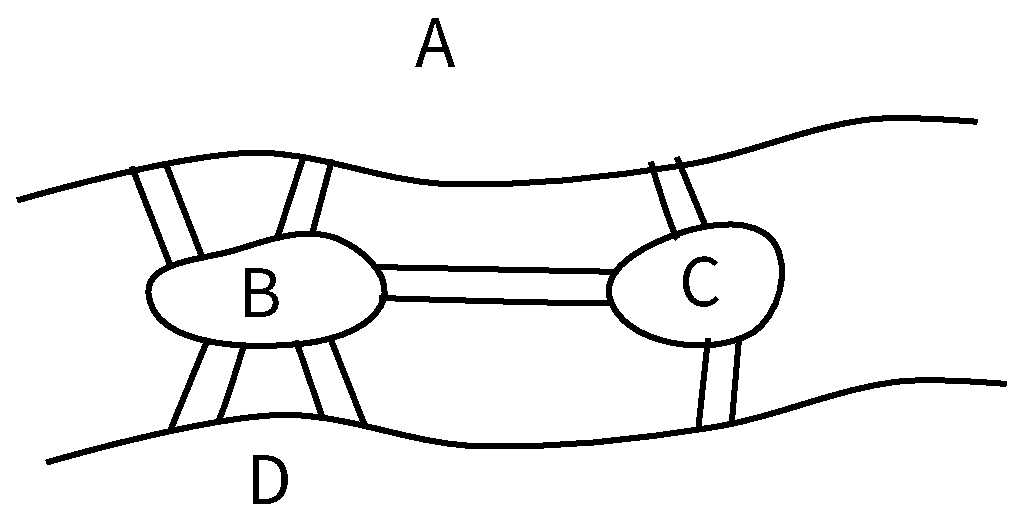
\includegraphics[width=5cm,height=4cm]{konigsberg}
\end{minipage}
 \pause
\hspace{1cm}\begin{minipage}{0.18\linewidth}
  \centering
  \begin{tikzpicture}[auto,
  specification/.style ={circle, draw, thick}, scale=0.8]
 \node[specification] (A) [label=270:D]  at (0,0)  {};
 \node[specification] (B) [label=180:B] at (0,2)  {};
 \node[specification] (C) [label=90:A]  at (0,4)  {};
 \node[specification] (D) [label=0:C]  at (2,2)  {};

 \draw[thick] (A) to [bend left=10] (B);
 \draw[thick] (A) to [bend right=10] (B);
 \draw[thick] (B) to [bend left=10]  (C);
 \draw[thick] (B) to [bend right=10]  (C);
 \draw[thick] (B) to [bend left=10]  (D);
 \draw[thick] (A) to   (D);
 \draw[thick] (C) to   (D);
 
\end{tikzpicture}
\end{minipage}

\end{frame}

\begin{frame}
  \frametitle{6.5 欧拉图}
\centering
\begin{minipage}{0.49\linewidth}
  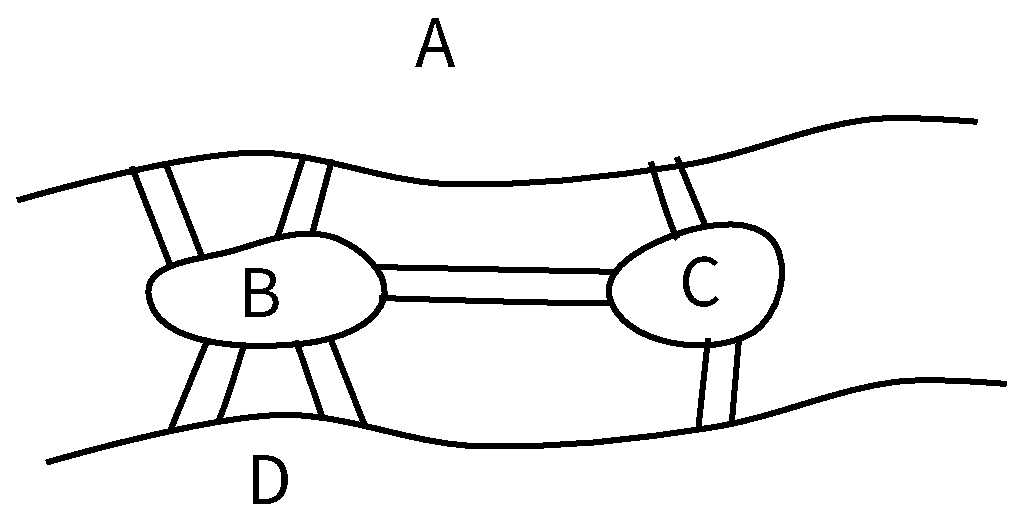
\includegraphics[width=5cm,height=4cm]{konigsberg}
\end{minipage}
 \pause
\hspace{1cm}\begin{minipage}{0.18\linewidth}
  \centering
  \begin{tikzpicture}[auto,
  specification/.style ={circle, draw, thick}, scale=0.8]
 \node[specification] (A) [label=270:D]  at (0,0)  {};
 \node[specification] (B) [label=180:B]  at (0,2)  {};
 \node[specification] (C) [label=90:A]  at (0,4)  {};
 \node[specification] (D) [label=0:C]  at (2,2)  {};

 \draw[thick] (A) to [bend left=10] (B);
 \draw[thick] (A) to [bend right=10] (B);
 \draw[thick] (B) to [bend left=10]  (C);
 \draw[thick] (B) to [bend right=10]  (C);
 \draw[thick] (B) to [bend left=10]  (D);
 \draw[thick] (B) to [bend right=10]  (D);
 \draw[thick] (A) to   (D);
 \draw[thick] (C) to   (D);
 \draw[thick] (A) to [bend left=60] (C);
 
\end{tikzpicture}
\end{minipage}

    \pause
  \begin{Def}
    包含图的所有顶点和所有边的闭迹称为\alert{欧拉闭迹}。存在一条欧拉闭迹的图称为\alert{欧拉图}。
  \end{Def}

\end{frame}
\begin{frame}
  \frametitle{6.5 欧拉图}
  \begin{Thm2}
    图G为欧拉图当且仅当$G$为连通的且每个顶点的度为偶数。
  \end{Thm2}\pause
  \centering\begin{minipage}{0.18\linewidth}\centering
    \begin{tikzpicture}[auto,
    specification/.style ={circle, draw, thick}, scale=0.8]
   \node[specification] (A) [label=270:D]  at (0,0)  {};
   \node[specification] (B) [label=180:B]  at (0,2)  {};
   \node[specification] (C) [label=90:A]  at (0,4)  {};
   \node[specification] (D) [label=0:C]  at (2,2)  {};
  
   \draw[thick] (A) to [bend left=10] (B);
   \draw[thick] (A) to [bend right=10] (B);
   \draw[thick] (B) to [bend left=10]  (C);
   \draw[thick] (B) to [bend right=10]  (C);
   \draw[thick] (B) to [bend left=10]  (D);
   \draw[thick] (B) to [bend right=10]  (D);
   \draw[thick] (A) to   (D);
   \draw[thick] (C) to   (D);
   \draw[thick] (A) to [bend left=60] (C);
   
  \end{tikzpicture}
  \end{minipage}
  
\end{frame}


\begin{frame}
  \frametitle{6.5 欧拉图}
  \begin{Thm}
    图G为欧拉图当且仅当$G$为连通的且每个顶点的度为偶数。
  \end{Thm}
\pause\begin{proof}[证明]\justifying\let\raggedright\justifying
      \pause首先,假设图$G$为欧拉图,往证$G$是连通的且每个顶点的度为偶数。

  \pause由图$G$为欧拉图知$G$中有一条包含所有边和所有顶点的闭迹$T:v_0,x_1,v_1,\ldots,
  x_n,v_n$,其中$v_n=v_0$。\pause显
  然$G$是连通的。\pause顶点$v_0$在$T$中的第一次出现与一条边相关联,\pause最后一次出现与一
  条边相关联,\pause其余的每次出现均与两条边相关联,\pause因此其度为偶数。\pause除$v_0$之外的其他
  顶点在$T$中的每次出现均与两条边相关联,\pause因此其度也为偶数。

  \end{proof}
\end{frame}

\begin{frame}
  \frametitle{6.5 欧拉图}
  \begin{Thm2}
    图G为欧拉图当且仅当$G$为连通的且每个顶点的度为偶数。
  \end{Thm2}
  \begin{proof}[证明(续上页)]
    \pause
    \centering\begin{minipage}{0.18\linewidth}\centering
      \begin{tikzpicture}[auto,
      specification/.style ={circle, draw, thick}, scale=0.8]
     \node[specification] (A) [label=270:D]  at (0,0)  {};
     \node[specification] (B) [label=180:B]  at (0,2)  {};
     \node[specification] (C) [label=90:A]  at (0,4)  {};
     \node[specification] (D) [label=0:C]  at (2,2)  {};
    
     \draw[thick] (A) to [bend left=10] (B);
     \draw[thick] (A) to [bend right=10] (B);
     \draw[thick] (B) to [bend left=10]  (C);
     \draw[thick] (B) to [bend right=10]  (C);
     \draw[thick] (B) to [bend left=10]  (D);
     \draw[thick] (B) to [bend right=10]  (D);
     \draw[thick] (A) to   (D);
     \draw[thick] (C) to   (D);
     \draw[thick] (A) to [bend left=60] (C);
     
    \end{tikzpicture}
    \end{minipage}
   
  \end{proof}
\end{frame}

\begin{frame}
  \frametitle{6.5 欧拉图}
  \begin{Thm2}
    图G为欧拉图当且仅当$G$为连通的且每个顶点的度为偶数。
  \end{Thm2}
  \begin{proof}[证明(续上页)]\justifying\let\raggedright\justifying
  \pause其次,\pause假设$G$为连通的且每个顶点的度为偶数,\pause往证$G$为欧拉图。

  \pause设$v_0,x_1,v_1,\ldots, x_n,v_n$为图$G$的一条最长的迹,\pause记为$Z$,\pause则$Z$为闭迹。\pause否
  则,\pause$v_n \neq v_0$,\pause$v_n$在迹$Z$中的最后一次出现与一条边相关联,\pause其他的每次出现
  均与两条边相关联,\pause由$v_n$的度为偶数知,\pause$v_n$在$G$中还有一条与之关联的边没有在
  $Z$中出现,\pause记为$x_{n+1}=v_nv_{n+1}$。\pause则$v_0,x_1,v_1,\ldots,
  x_n,v_n,x_{n+1},v_{n+1}$构成了图$G$的一条更长的迹,\pause这与$v_0,x_1,v_1,\ldots,
  x_n,v_n$为图$G$的一条最长的迹矛盾。\pause接下来证明$Z$包含了图$G$的所有的边。\pause若不然,
  \pause则图$G$中存在一条边$x$不在$Z$中出现,\pause并且$x$有一个端点在$Z$中出现。\pause在图$G$中去掉
  $Z$中的所有边,\pause得到图$G'$。\pause取图$G'$中一条包含$x$的最长的迹$Z'$,\pause由图$G'$中所有
  顶点的度均为偶数易知$Z'$为闭迹(与前面证明$Z$为闭迹的过程相类似)。\pause于是$Z$和
  $Z'$可以联结成一条更长的迹,\pause这与$v_0,x_1,v_1,\ldots, x_n,v_n$为图$G$的一条最长
  的迹矛盾。
  \end{proof}
\end{frame}

\begin{frame}
  \frametitle{6.5 欧拉图}
  \begin{Def}
    包含图的所有顶点和边的迹称为\alert{欧拉迹}。一条欧拉迹如果不是欧拉闭迹,则称其为\alert{欧拉开迹}。
  \end{Def}

\end{frame}

\begin{frame}
  \frametitle{6.5 欧拉图}
  \begin{Thm}
    图G有一条欧拉开迹当且仅当$G$为连通的且恰有两个奇度顶点。
  \end{Thm}
\pause\begin{proof}[证明]\justifying\let\raggedright\justifying
      \pause设图$G$有一条欧拉开迹$Z:v_0,x_1,v_1,\ldots, x_n,v_n$,\pause其中$x_i=v_{i-1}v_i, i =
  1,2,\ldots, n$。\pause显然,图$G$是连通的。\pause顶点$v_0$在$Z$中除了其首次出现与一条边相
  关联外,\pause其余的每次出现均与两
  条边相关联,\pause因此顶点$v_0$的度为奇数;\pause同理,\pause$v_n$的度为奇数。\pause除了$v_0$和$v_n$
  之外其余的每个顶点在$Z$中的每次出现均与两条边相关联,\pause因此其度为偶数。\pause这证明了
  图$G$恰有两个奇度顶点。

  \end{proof}
\end{frame}

\begin{frame}
  \frametitle{6.5 欧拉图}
  \begin{Thm5.2}
    图G有一条欧拉开迹当且仅当$G$为连通的且恰有两个奇度顶点。
  \end{Thm5.2}
\pause
\centering\begin{minipage}{0.18\linewidth}\centering
  \begin{tikzpicture}[auto,
  specification/.style ={circle, draw, thick}, scale=0.8]
 \node[specification] (A) [label=270:D]  at (0,0)  {};
 \node[specification] (B) [label=180:B]  at (0,2)  {};
 \node[specification] (C) [label=90:A]  at (0,4)  {};
 \node[specification] (D) [label=0:C]  at (2,2)  {};

 \draw[thick] (A) to [bend left=10] (B);
 \draw[thick] (A) to [bend right=10] (B);
 \draw[thick] (B) to [bend left=10]  (C);
 \draw[thick] (B) to [bend right=10]  (C);
 \draw[thick] (B) to [bend left=10]  (D);
 \draw[thick] (B) to [bend right=10]  (D);
 \draw[thick] (A) to   (D);
 \draw[thick] (C) to   (D);
 
\end{tikzpicture}
\end{minipage}

\end{frame}

\begin{frame}
  \frametitle{6.5 欧拉图}
  \begin{Thm5.2}
    图G有一条欧拉开迹当且仅当$G$为连通的且恰有两个奇度顶点。
  \end{Thm5.2}
\pause\begin{proof}[证明]\justifying\let\raggedright\justifying
      

  \pause设图$G$是连通的,\pause且恰有两个奇度顶点$u$和$v$。\pause在顶点$u$和$v$之间加一条边,\pause得
  到图$G'$。\pause则图$G'$是连通的且每个顶点的度为偶数,\pause因此有一条欧拉闭迹。\pause在该欧拉闭迹上去掉
  新加的顶点$u$与顶点$v$之间的边,\pause便得到了图$G$的一条欧拉开迹。
  \end{proof}
\end{frame}
\begin{frame}
  \frametitle{6.5 欧拉图}
  \begin{Thm5.3}
    设$G$为连通图,$G$恰有$2n$个奇度顶点,$n \geq 1$,则$G$的全部边可以排成$n$条
    开迹,且不能排成少于$n$条开迹。  \end{Thm5.3}
\pause 
\pause
\centering\begin{minipage}{0.18\linewidth}\centering
  \begin{tikzpicture}[auto,
  specification/.style ={circle, draw, thick}, scale=0.8]
 \node[specification] (A) [label=270:D]  at (0,0)  {};
 \node[specification] (B) [label=180:B]  at (0,2)  {};
 \node[specification] (C) [label=90:A]  at (0,4)  {};
 \node[specification] (D) [label=0:C]  at (2,2)  {};

 \draw[thick] (A) to [bend left=10] (B);
 \draw[thick] (A) to [bend right=10] (B);
 \draw[thick] (B) to [bend left=10]  (C);
 \draw[thick] (B) to [bend right=10]  (C);
 \draw[thick] (B) to [bend left=10]  (D);
 \draw[thick] (A) to   (D);
 \draw[thick] (C) to   (D);
 
\end{tikzpicture}
\end{minipage}

\end{frame}

\begin{frame}
  \frametitle{6.5 欧拉图}
  \begin{Thm}
    设$G$为连通图,$G$恰有$2n$个奇度顶点,$n \geq 1$,则$G$的全部边可以排成$n$条
    开迹,且不能排成少于$n$条开迹。  \end{Thm}
\pause  \begin{proof}[证明]\justifying\let\raggedright\justifying
      \pause设连通图$G$有$2n$个奇度顶点$u_1,v_1,u_2,v_2,\ldots,u_n,v_n$。\pause在$G$中加
  入$n$条边$u_1v_1$, $u_2v_2$, $\ldots$, $u_nv_n$,\pause得到图$G'$。\pause则$G'$是连通的,
  \pause且每个顶点的度为偶数,\pause因此存在一条欧拉闭迹$Z$。\pause在$Z$中去掉新加入的边$u_1v_1,
  u_2v_2, \ldots, u_nv_n$,\pause则得到图$G$的$n$条开迹。

  \pause假设图$G$的所有边能排成$m$条开迹,\pause$m < n$。\pause则只有这$m$条开迹的端点可能为
  奇度顶点,\pause因此图$G$至多有$2m$个奇度顶点,\pause这与图$G$有$2n$个奇度顶点矛盾。
  \end{proof}
\end{frame}
\begin{frame}
  包含图的所有顶点和所有边的闭迹称为\alert{欧拉闭迹}。存在一条欧拉闭迹的图称为\alert{欧拉图}。

  \centering
  \begin{minipage}{0.24\linewidth}
    \centering
    \begin{tikzpicture}[auto,
    specification/.style ={circle, draw, thick}]
   \node[specification] (A) at (0,0)  {};
   \node[specification] (B)  at (0,1)  {};
   \node[specification] (C)  at (1,1)  {};
   \node[specification] (D) at (1,0)  {};
 \end{tikzpicture}\\
 \vspace*{0.1cm}
 A
\end{minipage}\hfill 
  \begin{minipage}{0.24\linewidth}
    \centering
    \begin{tikzpicture}[auto,
    specification/.style ={circle, draw, thick}]
   \node[specification] (A) at (0,0)  {};
   \node[specification] (B) at (0,1)  {};
   \node[specification] (C) at (1,1)  {};
   \node[specification] (D) at (1,0)  {};
   \draw[thick] (B) to  (C);
 \end{tikzpicture}\\
 \vspace*{0.1cm}
 B
\end{minipage}\hfill 
  \begin{minipage}{0.24\linewidth}
    \centering
    \begin{tikzpicture}[auto,
    specification/.style ={circle, draw, thick}]
   \node[specification] (A) at (0,0)  {};
   \node[specification] (B) at (0,1)  {};
   \node[specification] (C) at (1,1)  {};
   \node[specification] (D) at (1,0)  {};
   \draw[thick] (A) to  (B);
   \draw[thick] (B) to  (C);
 \end{tikzpicture}\\
 \vspace*{0.1cm}
 C
\end{minipage}\hfill 
  \begin{minipage}{0.24\linewidth}
    \centering
    \begin{tikzpicture}[auto,
    specification/.style ={circle, draw, thick}]
   \node[specification] (A)  at (0,0)  {};
   \node[specification] (B)  at (0,1)  {};
   \node[specification] (C)  at (1,1)  {};
   \node[specification] (D) at (1,0)  {};
   \draw[thick] (B) to  (C);
   \draw[thick] (D) to  (A);
 \end{tikzpicture}\\
 \vspace*{0.1cm}
 D
\end{minipage}\hfill

\vspace*{0.5cm}
  \begin{minipage}{0.24\linewidth}
    \centering
    \begin{tikzpicture}[auto,
    specification/.style ={circle, draw, thick}]
   \node[specification] (A) at (0,0)  {};
   \node[specification] (B)  at (0,1)  {};
   \node[specification] (C)  at (1,1)  {};
   \node[specification] (D) at (1,0)  {};
   \draw[thick] (A) to (B);
   \draw[thick] (B) to (C);
      \draw[thick] (B) to (D);
 \end{tikzpicture}\\
 \vspace*{0.1cm}
 E
\end{minipage}\hfill
  \begin{minipage}{0.24\linewidth}
    \centering
    \begin{tikzpicture}[auto,
    specification/.style ={circle, draw, thick}]
   \node[specification] (A) at (0,0)  {};
   \node[specification] (B) at (0,1)  {};
   \node[specification] (C) at (1,1)  {};
   \node[specification] (D) at (1,0)  {};
   \draw[thick] (A) to  (B);
   \draw[thick] (B) to (C);
   \draw[thick] (C) to (A);
 \end{tikzpicture}\\
 \vspace*{0.1cm}
 F
\end{minipage}\hfill
  \begin{minipage}{0.24\linewidth}
    \centering
    \begin{tikzpicture}[auto,
    specification/.style ={circle, draw, thick}]
   \node[specification] (A) at (0,0)  {};
   \node[specification] (B) at (0,1)  {};
   \node[specification] (C) at (1,1)  {};
   \node[specification] (D) at (1,0)  {};
   \draw[thick] (A) to  (B);
   \draw[thick] (B) to  (C);
      \draw[thick] (C) to (D);
 \end{tikzpicture}\\
 \vspace*{0.1cm}
 G
\end{minipage}\hfill 
  \begin{minipage}{0.24\linewidth}
    \centering
    \begin{tikzpicture}[auto,
    specification/.style ={circle, draw, thick}]
   \node[specification] (A)  at (0,0)  {};
   \node[specification] (B)  at (0,1)  {};
   \node[specification] (C)  at (1,1)  {};
   \node[specification] (D) at (1,0)  {};
   \draw[thick] (A) to  (C);
   \draw[thick] (C) to  (D);
   \draw[thick] (D) to (A);
   \draw[thick] (B) to (D);
 \end{tikzpicture}\\
 \vspace*{0.1cm}
 H
\end{minipage}\hfill 

\vspace*{0.5cm}
\flushleft
  \begin{minipage}{0.24\linewidth}
    \centering
    \begin{tikzpicture}[auto,
    specification/.style ={circle, draw, thick}]
   \node[specification] (A) at (0,0)  {};
   \node[specification] (B)  at (0,1)  {};
   \node[specification] (C)  at (1,1)  {};
   \node[specification] (D) at (1,0)  {};
   \draw[thick] (A) to (B);
   \draw[thick] (B) to (D);
   \draw[thick] (D) to (C);
      \draw[thick] (C) to (A);
 \end{tikzpicture}\\
 \vspace*{0.1cm}
 I
\end{minipage}
  \begin{minipage}{0.24\linewidth}
    \centering
    \begin{tikzpicture}[auto,
    specification/.style ={circle, draw, thick}]
   \node[specification] (A) at (0,0)  {};
   \node[specification] (B) at (0,1)  {};
   \node[specification] (C) at (1,1)  {};
   \node[specification] (D) at (1,0)  {};
   \draw[thick] (A) to  (B);
      \draw[thick] (C) to (D);
   \draw[thick] (D) to (A);
   \draw[thick] (A) to (C);
   \draw[thick] (B) to (D);
 \end{tikzpicture}\\
 \vspace*{0.1cm}
 J
\end{minipage} 
  \begin{minipage}{0.24\linewidth}
    \centering
    \begin{tikzpicture}[auto,
    specification/.style ={circle, draw, thick}]
   \node[specification] (A) at (0,0)  {};
   \node[specification] (B) at (0,1)  {};
   \node[specification] (C) at (1,1)  {};
   \node[specification] (D) at (1,0)  {};
   \draw[thick] (A) to  (B);
   \draw[thick] (B) to  (C);
      \draw[thick] (C) to (D);
   \draw[thick] (D) to (A);
   \draw[thick] (A) to (C);
   \draw[thick] (B) to (D);
 \end{tikzpicture}\\
 \vspace*{0.1cm}
 K
\end{minipage}  
\end{frame}
% \begin{frame}
%   \frametitle{6.6 哈密顿图}
% \centering
% \includegraphics[width=5cm,height=4cm]{hamiltonian} 
%  \pause
%   \begin{definition6.6.1}
%     图$G$的一条包含所有顶点的路称为$G$的一条\alert{哈密顿路};图$G$的一个包含所有顶点的圈称为$G$的一个\alert{哈密顿圈}。具有哈密顿圈的图称为\alert{哈密顿图}。
%   \end{definition6.6.1}
% \end{frame}

\section{哈密顿图}
\begin{frame}
  \frametitle{6.6 哈密顿图}
  \centering
    \begin{tikzpicture}[auto,
    specification/.style ={circle, draw, thick, inner sep = 0pt, minimum size=2mm}]
   \node[specification] (A)  at (18:2.3cm)  {};
   \node[specification] (B)  at (90:2.3cm)  {};
   \node[specification] (C)  at (162:2.3cm)  {};
   \node[specification] (D) at (234:2.3cm)  {};
   \node[specification] (E)  at (306:2.3cm)  {};
   \node[specification] (F)  at (18:1.5cm)  {};
   \node[specification] (G)  at (90:1.5cm)  {};
   \node[specification] (H)  at (162:1.5cm)  {};
   \node[specification] (I) at (234:1.5cm)  {};
   \node[specification] (J)  at (306:1.5cm)  {};
   \node[specification] (K)  at (-18:1.0cm)  {};
   \node[specification] (L)  at (-90:1.0cm)  {};
   \node[specification] (M)  at (-162:1.0cm)  {};
   \node[specification] (N) at (-234:1.0cm)  {};
   \node[specification] (O)  at (-306:1.0cm)  {};
   \node[specification] (P)  at (-18:0.5cm)  {};
   \node[specification] (Q)  at (-90:0.5cm)  {};
   \node[specification] (R)  at (-162:0.5cm)  {};
   \node[specification] (S) at (-234:0.5cm)  {};
   \node[specification] (T)  at (-306:0.5cm)  {};
   
   
   \draw[thick] (A) to  (B);
   \draw[thick] (B) to  (C);
   \draw[thick] (C) to  (D);
   \draw[thick] (D) to  (E);
   \draw[thick] (E) to  (A);
   \draw[thick] (A) to  (F);
   \draw[thick] (B) to  (G);
   \draw[thick] (C) to  (H);
   \draw[thick] (D) to  (I);
   \draw[thick] (E) to  (J);

   \draw[thick] (F) to  (O);
   \draw[thick] (O) to  (G);
   \draw[thick] (G) to  (N);
   \draw[thick] (N) to  (H);
   \draw[thick] (H) to  (M);
   \draw[thick] (M) to  (I);
   \draw[thick] (I) to  (L);
   \draw[thick] (L) to  (J);
   \draw[thick] (J) to  (K);
   \draw[thick] (K) to  (F);

   \draw[thick] (P) to  (K);
   \draw[thick] (Q) to  (L);
   \draw[thick] (R) to  (M);
   \draw[thick] (S) to  (N);
   \draw[thick] (T) to  (O);

   \draw[thick] (P) to  (Q);
   \draw[thick] (Q) to  (R);
   \draw[thick] (R) to  (S);
   \draw[thick] (S) to  (T);
   \draw[thick] (T) to  (P);
 \end{tikzpicture}
\end{frame}

\begin{frame}
  \frametitle{6.6 哈密顿图}
   \begin{Def}
    图$G$的一条包含所有顶点的路称为$G$的一条\alert{哈密顿路};图$G$的一个包含所有顶点的圈称为$G$的一个\alert{哈密顿圈}。具有哈密顿圈的图称为\alert{哈密顿图}。
  \end{Def}  
\end{frame}

\begin{frame}
  \frametitle{6.6 哈密顿图}
  \centering
    \begin{tikzpicture}[auto,
    specification/.style ={circle, draw, thick, inner sep = 0pt, minimum size=2mm}]
   \node[specification] (A)  at (30:2.3cm)  {};
   \node[specification] (B)  at (90:2.3cm)  {};
   \node[specification] (C)  at (150:2.3cm)  {};
   \node[specification] (D) at (210:2.3cm)  {};
   \node[specification] (E)  at (270:2.3cm)  {};
   \node[specification] (F)  at (330:2.3cm)  {};
   \node[specification] (G)  at (30:1.5cm)  {};
   \node[specification] (H)  at (90:1.5cm)  {};
   \node[specification] (I) at (150:1.5cm)  {};
   \node[specification] (J)  at (210:1.5cm)  {};
   \node[specification] (K)  at (270:1.5cm)  {};
   \node[specification] (L)  at (330:1.5cm)  {};
   \node[specification] (M)  at (30:0.75cm)  {};
   \node[specification] (N)  at (150:0.75cm)  {};
   \node[specification] (P)  at (270:0.75cm)  {};
   \node[specification] (Q)  at (0,0)  {};
   \draw[thick] (A) to  (B);
   \draw[thick] (B) to  (C);
   \draw[thick] (C) to  (D);
   \draw[thick] (D) to  (E);
   \draw[thick] (E) to  (F);
   \draw[thick] (F) to  (A);
   \draw[thick] (A) to  (G);
   \draw[thick] (B) to  (H);
   \draw[thick] (C) to  (I);
   \draw[thick] (D) to  (J);
   \draw[thick] (E) to  (K);
   \draw[thick] (F) to  (L);
   \draw[thick] (G) to  (H);
   \draw[thick] (H) to  (I);
   \draw[thick] (I) to  (J);
   \draw[thick] (J) to  (K);
   \draw[thick] (K) to  (L);
   \draw[thick] (L) to  (G);
   \draw[thick] (H) to  (M);
   \draw[thick] (M) to  (L);
   \draw[thick] (L) to  (P);
   \draw[thick] (P) to  (J);
   \draw[thick] (J) to  (N);
   \draw[thick] (N) to  (H);
   \draw[thick] (M) to  (Q);
   \draw[thick] (N) to  (Q);
   \draw[thick] (P) to  (Q);
 \end{tikzpicture}
\end{frame}
\begin{frame}[t]
  \frametitle{6.6 哈密顿图}
  \centering
  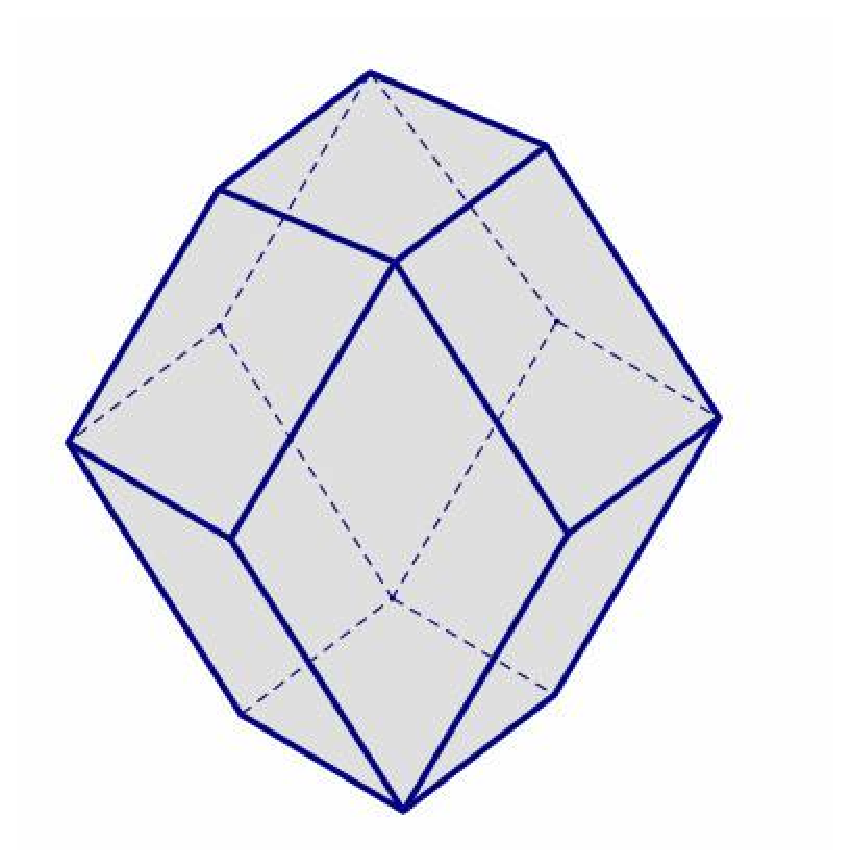
\includegraphics[width=5cm,height=4cm]{timg}
\end{frame}

\begin{frame}
  \frametitle{6.6 哈密顿图}
  \begin{Thm}
    设$G=(V,E)$为哈密顿图,则对$V$的每个非空子集$S$,均有
    \[\omega(G-S) \leq |S|\]
    其中$G-S$是从$G$中去掉$S$中那些顶点后所得到的图,$\omega(G-S)$是图$G-S$的支数。
  \end{Thm}
\end{frame}

\begin{frame}
  \frametitle{6.6 哈密顿图}
  \centering
    \begin{tikzpicture}[auto,
    specification/.style ={circle, draw, thick, inner sep = 0pt, minimum size=2mm}]
   \node[specification] (A)  at (90:1.6cm)  {};
   \node[specification] (B)  at (210:1.6cm)  {};
   \node[specification] (C)  at (330:1.6cm)  {};
   \node[specification] (D)  at (90:0.8cm)  {};
   \node[specification] (E)  at (210:0.8cm)  {};
   \node[specification] (F)  at (330:0.8cm)  {};
   \node[specification] (G)  at (210:2.4cm)  {};
   \node[specification] (H)  at (330:2.4cm)  {};
   \node[specification] (I)  at (0,0)  {};
   
   
   \draw[thick] (A) to  (B);
   \draw[thick] (B) to  (C);
   \draw[thick] (C) to  (A);
   \draw[thick] (D) to  (E);
   \draw[thick] (E) to  (F);
   \draw[thick] (F) to  (D);
   \draw[thick] (D) to  (G);
   \draw[thick] (D) to  (H);
   \draw[thick] (H) to  (B);
   \draw[thick] (G) to  (C);
   \draw[thick] (A) to  (D);
   \draw[thick] (C) to  (F);
   \draw[thick] (B) to  (E);
   \draw[thick] (I) to  (D);
   \draw[thick] (I) to  (E);
   \draw[thick] (I) to  (F);
   \draw[thick] (G) to  (B);
   \draw[thick] (H) to  (C);
   \draw[thick] (B) to [bend right = 10] (I);
   \draw[thick] (C) to [bend left = 10] (I);
 \end{tikzpicture}
\end{frame}
\begin{frame}
  \frametitle{6.6 哈密顿图}
  \centering
    \begin{tikzpicture}[auto,
    specification/.style ={circle, draw, thick, inner sep = 0pt, minimum size=2mm}]
   \node[specification] (A)  at (18:2.3cm)  {};
   \node[specification] (B)  at (90:2.3cm)  {};
   \node[specification] (C)  at (162:2.3cm)  {};
   \node[specification] (D) at (234:2.3cm)  {};
   \node[specification] (E)  at (306:2.3cm)  {};
   \node[specification] (F)  at (18:1.5cm)  {};
   \node[specification] (G)  at (90:1.5cm)  {};
   \node[specification] (H)  at (162:1.5cm)  {};
   \node[specification] (I) at (234:1.5cm)  {};
   \node[specification] (J) at (306:1.5cm)  {};
   
   
   \draw[thick] (A) to  (B);
   \draw[thick] (B) to  (C);
   \draw[thick] (C) to  (D);
   \draw[thick] (D) to  (E);
   \draw[thick] (E) to  (A);
   \draw[thick] (A) to  (F);
   \draw[thick] (B) to  (G);
   \draw[thick] (C) to  (H);
   \draw[thick] (D) to  (I);
   \draw[thick] (E) to  (J);

   \draw[thick] (F) to  (H);
   \draw[thick] (H) to  (J);
   \draw[thick] (J) to  (G);
   \draw[thick] (G) to  (I);
   \draw[thick] (I) to  (F);
 \end{tikzpicture}
\end{frame}

\begin{frame}
    \centering
  \begin{minipage}{0.24\linewidth}
    \centering
    \begin{tikzpicture}[auto,
    specification/.style ={circle, draw, thick}]
   \node[specification] (A) at (0,0)  {};
   \node[specification] (B)  at (0,1)  {};
   \node[specification] (C)  at (1,1)  {};
   \node[specification] (D) at (1,0)  {};
 \end{tikzpicture}\\
 \vspace*{0.1cm}
 A
\end{minipage}\hfill 
  \begin{minipage}{0.24\linewidth}
    \centering
    \begin{tikzpicture}[auto,
    specification/.style ={circle, draw, thick}]
   \node[specification] (A) at (0,0)  {};
   \node[specification] (B) at (0,1)  {};
   \node[specification] (C) at (1,1)  {};
   \node[specification] (D) at (1,0)  {};
   \draw[thick] (B) to  (C);
 \end{tikzpicture}\\
 \vspace*{0.1cm}
 B
\end{minipage}\hfill 
  \begin{minipage}{0.24\linewidth}
    \centering
    \begin{tikzpicture}[auto,
    specification/.style ={circle, draw, thick}]
   \node[specification] (A) at (0,0)  {};
   \node[specification] (B) at (0,1)  {};
   \node[specification] (C) at (1,1)  {};
   \node[specification] (D) at (1,0)  {};
   \draw[thick] (A) to  (B);
   \draw[thick] (B) to  (C);
 \end{tikzpicture}\\
 \vspace*{0.1cm}
 C
\end{minipage}\hfill 
  \begin{minipage}{0.24\linewidth}
    \centering
    \begin{tikzpicture}[auto,
    specification/.style ={circle, draw, thick}]
   \node[specification] (A)  at (0,0)  {};
   \node[specification] (B)  at (0,1)  {};
   \node[specification] (C)  at (1,1)  {};
   \node[specification] (D) at (1,0)  {};
   \draw[thick] (B) to  (C);
   \draw[thick] (D) to  (A);
 \end{tikzpicture}\\
 \vspace*{0.1cm}
 D
\end{minipage}\hfill

\vspace*{0.5cm}
  \begin{minipage}{0.24\linewidth}
    \centering
    \begin{tikzpicture}[auto,
    specification/.style ={circle, draw, thick}]
   \node[specification] (A) at (0,0)  {};
   \node[specification] (B)  at (0,1)  {};
   \node[specification] (C)  at (1,1)  {};
   \node[specification] (D) at (1,0)  {};
   \draw[thick] (A) to (B);
   \draw[thick] (B) to (C);
      \draw[thick] (B) to (D);
 \end{tikzpicture}\\
 \vspace*{0.1cm}
 E
\end{minipage}\hfill
  \begin{minipage}{0.24\linewidth}
    \centering
    \begin{tikzpicture}[auto,
    specification/.style ={circle, draw, thick}]
   \node[specification] (A) at (0,0)  {};
   \node[specification] (B) at (0,1)  {};
   \node[specification] (C) at (1,1)  {};
   \node[specification] (D) at (1,0)  {};
   \draw[thick] (A) to  (B);
   \draw[thick] (B) to (C);
   \draw[thick] (C) to (A);
 \end{tikzpicture}\\
 \vspace*{0.1cm}
 F
\end{minipage}\hfill
  \begin{minipage}{0.24\linewidth}
    \centering
    \begin{tikzpicture}[auto,
    specification/.style ={circle, draw, thick}]
   \node[specification] (A) at (0,0)  {};
   \node[specification] (B) at (0,1)  {};
   \node[specification] (C) at (1,1)  {};
   \node[specification] (D) at (1,0)  {};
   \draw[thick] (A) to  (B);
   \draw[thick] (B) to  (C);
      \draw[thick] (C) to (D);
 \end{tikzpicture}\\
 \vspace*{0.1cm}
 G
\end{minipage}\hfill 
  \begin{minipage}{0.24\linewidth}
    \centering
    \begin{tikzpicture}[auto,
    specification/.style ={circle, draw, thick}]
   \node[specification] (A)  at (0,0)  {};
   \node[specification] (B)  at (0,1)  {};
   \node[specification] (C)  at (1,1)  {};
   \node[specification] (D) at (1,0)  {};
   \draw[thick] (A) to  (C);
   \draw[thick] (C) to  (D);
   \draw[thick] (D) to (A);
   \draw[thick] (B) to (D);
 \end{tikzpicture}\\
 \vspace*{0.1cm}
 H
\end{minipage}\hfill 

\vspace*{0.5cm}
\flushleft
  \begin{minipage}{0.24\linewidth}
    \centering
    \begin{tikzpicture}[auto,
    specification/.style ={circle, draw, thick}]
   \node[specification] (A) at (0,0)  {};
   \node[specification] (B)  at (0,1)  {};
   \node[specification] (C)  at (1,1)  {};
   \node[specification] (D) at (1,0)  {};
   \draw[thick] (A) to (B);
   \draw[thick] (B) to (D);
   \draw[thick] (D) to (C);
      \draw[thick] (C) to (A);
 \end{tikzpicture}\\
 \vspace*{0.1cm}
 I
\end{minipage}
  \begin{minipage}{0.24\linewidth}
    \centering
    \begin{tikzpicture}[auto,
    specification/.style ={circle, draw, thick}]
   \node[specification] (A) at (0,0)  {};
   \node[specification] (B) at (0,1)  {};
   \node[specification] (C) at (1,1)  {};
   \node[specification] (D) at (1,0)  {};
   \draw[thick] (A) to  (B);
      \draw[thick] (C) to (D);
   \draw[thick] (D) to (A);
   \draw[thick] (A) to (C);
   \draw[thick] (B) to (D);
 \end{tikzpicture}\\
 \vspace*{0.1cm}
 J
\end{minipage} 
  \begin{minipage}{0.24\linewidth}
    \centering
    \begin{tikzpicture}[auto,
    specification/.style ={circle, draw, thick}]
   \node[specification] (A) at (0,0)  {};
   \node[specification] (B) at (0,1)  {};
   \node[specification] (C) at (1,1)  {};
   \node[specification] (D) at (1,0)  {};
   \draw[thick] (A) to  (B);
   \draw[thick] (B) to  (C);
      \draw[thick] (C) to (D);
   \draw[thick] (D) to (A);
   \draw[thick] (A) to (C);
   \draw[thick] (B) to (D);
 \end{tikzpicture}\\
 \vspace*{0.1cm}
 K
\end{minipage}  
\end{frame}

\begin{frame}
  \frametitle{6.6 哈密顿图}
  \begin{Thm3}
    设$G$为有$p(p \geq 3)$个顶点的图。如果对$G$的任一对不邻接的顶点$u$和$v$,均有
    \begin{equation*}
      \deg u + \deg v \geq p,
    \end{equation*}
则$G$是一个哈密顿图。
  \end{Thm3}
\end{frame}
\begin{frame}
  \frametitle{6.6 哈密顿图}
  \begin{Thm}
    设$G$为一个有$p$个顶点的图,如果对$G$的每一对不临接的顶点$u$和$v$,均有
    \begin{equation*}
      \deg u + \deg v \geq p - 1,
    \end{equation*}
则$G$为连通的。
\end{Thm}

\end{frame}

\begin{frame}
  \frametitle{6.6 哈密顿图}
  \begin{Thm}\label{hamilton path}
    设$G$为一个有$p$个顶点的图,如果对$G$的每一对不临接的顶点$u$和$v$,均有
    \begin{equation*}
      \deg u + \deg v \geq p - 1,
    \end{equation*}
则$G$有哈密顿路。
\end{Thm}
\centering
\vspace{0.5cm}
    \begin{tikzpicture}[auto,
    specification/.style ={circle, draw, thick, inner sep = 0pt, minimum size=2mm}]
   \node[specification] (A)  [label=-90:$v_1$] at (0,0)  {};
   \node[specification] (B)  [label=-90:$v_2$] at (0.5,0)  {};
   \node[specification] (C)  at (1,0)  {};
   \node[specification] (D) at (1.5,0)  {};
   \node[specification] (E)  [label=-90:$v_{i_{s-1}}$] at (2,0)  {};
   \node[specification] (F)  [label=-90:$v_{i_s}$]at (2.5,0)  {};
   \node[specification] (G)  at (3,0)  {};
   \node[specification] (H)  at (3.5,0)  {};
   \node[specification] (I) at (4,0)  {};
   \node[specification] (J) [label=-90:$v_{k-1}$] at (4.5,0)  {};
   \node[specification] (K) [label=-90:$v_k$] at (5,0)  {};
   
   
   \draw[thick] (A) to  (B);
   \draw[thick] (B) to  (C);
   \draw[thick] (C) to  (D);
   \draw[thick] (D) to  (E);
   \draw[thick] (E) to  (F);
   \draw[thick] (F) to  (G);
   \draw[thick] (G) to  (H);
   \draw[thick] (H) to  (I);
   \draw[thick] (I) to  (J);
   \draw[thick] (J) to  (K);
%   \draw[thick] (A) to [bend left = 20] (F);
%   \draw[thick] (K) to [bend left = 20] (E);
 \end{tikzpicture}
   \small{
     \pause\begin{proof}[证明]
          \pause当$p=1,2,3$时,易验证结论成立。\pause以下证明当$p\geq 4$时结论成立。

    \pause设$G$中的最长路为$v_1v_2\cdots v_k$,\pause 只需证明$k = p$。\pause

    用反证法,假设$k < p$。 \pause 易验证此时$k\geq 3$。\pause 以下证明$v_1v_2\cdots v_k$必在同一个圈上。\pause
    由$v_1v_2\cdots v_k$为最长路知$v_1$只能与$v_2,v_3,\ldots,v_{k-1},v_k$中的顶点邻接,\pause$v_k$只能与$v_1,v_2,v_3,\ldots,v_{k-1}$中的顶点邻接。
    % \begin{itemize}
    % \item 如果$v_1$与$v_k$邻接,则$v_1v_2\cdots v_kv_1$构成$G$中的一个圈;\pause
    % \item 如果$v_1$与$v_k$不邻接,由$v_1v_2\cdots v_k$为最长路知$v_1,v_k$只能与$v_2,v_3,\ldots,v_{k-1}$中的顶点邻接。
    % \end{itemize}

    \renewcommand{\qedsymbol}{}    
\end{proof}
}

\end{frame}

\begin{frame}
  \frametitle{6.6 哈密顿图}
  \begin{Thm1}
    设$G$为一个有$p$个顶点的图,如果对$G$的每一对不临接的顶点$u$和$v$,均有
    \begin{equation*}
      \deg u + \deg v \geq p - 1,
    \end{equation*}
则$G$有哈密顿路。
\end{Thm1}
\centering
\vspace{0.5cm}
    \begin{tikzpicture}[auto,
    specification/.style ={circle, draw, thick, inner sep = 0pt, minimum size=2mm}]
   \node[specification] (A)  [label=-90:$v_1$] at (0,0)  {};
   \node[specification] (B)  [label=-90:$v_2$] at (0.5,0)  {};
   \node[specification] (C)  at (1,0)  {};
   \node[specification] (D) at (1.5,0)  {};
   \node[specification] (E)  [label=-90:$v_{i_{s-1}}$] at (2,0)  {};
   \node[specification] (F)  [label=-90:$v_{i_s}$]at (2.5,0)  {};
   \node[specification] (G)  at (3,0)  {};
   \node[specification] (H)  at (3.5,0)  {};
   \node[specification] (I) at (4,0)  {};
   \node[specification] (J) [label=-90:$v_{k-1}$] at (4.5,0)  {};
   \node[specification] (K) [label=-90:$v_k$] at (5,0)  {};
   
   
   \draw[thick] (A) to  (B);
   \draw[thick] (B) to  (C);
   \draw[thick] (C) to  (D);
   \draw[thick] (D) to  (E);
   \draw[thick] (E) to  (F);
   \draw[thick] (F) to  (G);
   \draw[thick] (G) to  (H);
   \draw[thick] (H) to  (I);
   \draw[thick] (I) to  (J);
   \draw[thick] (J) to  (K);
   \draw[thick] (A) to [bend left = 20] (F);
   \draw[thick] (K) to [bend left = 20] (E);
 \end{tikzpicture}
 \small{
 \begin{proof}[证明(续上页)]
   \pause设$v_{i_1},v_{i_2},\ldots,v_{i_r}$与$v_1$邻接,\pause$2=i_1 < i_2 < \cdots < i_r \leq k$,\pause则$v_k$必与某个$v_{i_s-1}$邻接。
      \pause否则,\pause$v_k$至多与最长路上其余的顶点邻接,\pause所以
      \[\deg v_1 + \deg v_k \leq r + ((k-1) - r) = k - 1 < p - 1\]
      \pause矛盾。\pause于是,\pause$v_1v_2\cdots v_{i_{s-1}}v_kv_{k-1}\cdots v_{i_s}v_1$为$G$中的一个圈。
      % 总之,$v_1,v_2,\cdots,v_k$在$G$的同一个圈$C$上。
  \renewcommand{\qedsymbol}{}        
  \end{proof}
}

\end{frame}

\begin{frame}
  \frametitle{6.6 哈密顿图}
  \begin{Thm1}
    设$G$是一个有$p$个顶点的图,如果对$G$的每一对不临接的顶点$u$和$v$,均有
    \begin{equation*}
      \deg u + \deg v \geq p - 1,
    \end{equation*}
则$G$有哈密顿路。
\end{Thm1}
\centering
\vspace{0.5cm}
    \begin{tikzpicture}[auto,
    specification/.style ={circle, draw, thick, inner sep = 0pt, minimum size=2mm}]
   \node[specification] (A)  [label=-90:$v_1$] at (0,0)  {};
   \node[specification] (B)  [label=-90:$v_2$] at (0.5,0)  {};
   \node[specification] (C)  at (1,0)  {};
   \node[specification] (D) at (1.5,0)  {};
   \node[specification] (E)  [label=-90:$v_{i_{s-1}}$] at (2,0)  {};
   \node[specification] (F)  [label=-90:$v_{i_s}$]at (2.5,0)  {};
   \node[specification] (G)  at (3,0)  {};
   \node[specification] (H)  at (3.5,0)  {};
   \node[specification] (I) at (4,0)  {};
   \node[specification] (J) [label=-90:$v_{k-1}$] at (4.5,0)  {};
   \node[specification] (K) [label=-90:$v_k$] at (5,0)  {};
   
   
   \draw[thick] (A) to  (B);
   \draw[thick] (B) to  (C);
   \draw[thick] (C) to  (D);
   \draw[thick] (D) to  (E);
   \draw[thick] (E) to  (F);
   \draw[thick] (F) to  (G);
   \draw[thick] (G) to  (H);
   \draw[thick] (H) to  (I);
   \draw[thick] (I) to  (J);
   \draw[thick] (J) to  (K);
   \draw[thick] (A) to [bend left = 20] (F);
   \draw[thick] (K) to [bend left = 20] (E);
 \end{tikzpicture}
 \small{
 \begin{proof}[证明(续上页)]    
    \pause由于$G$为连通的,\pause$k < p$,\pause所以$G$必有某个顶点$v$,\pause$v$不在$C$上,\pause但
    与$C$上某个顶点$v_i$邻接。\pause于是得到$G$的一条更长的路,\pause这就出现了矛盾。
    
  \end{proof}
}

\end{frame}

\begin{frame}
  \frametitle{6.6 哈密顿图}
  \begin{Thm}
    设$G$为有$p(p \geq 3)$个顶点的图。如果对$G$的任一对不邻接的顶点$u$和$v$,均有
    \begin{equation*}
      \deg u + \deg v \geq p,
    \end{equation*}
则$G$是一个哈密顿图。
\end{Thm}
\centering
\vspace{0.5cm}
    \begin{tikzpicture}[auto,
    specification/.style ={circle, draw, thick, inner sep = 0pt, minimum size=2mm}]
   \node[specification] (A)  [label=-90:$v_1$] at (0,0)  {};
   \node[specification] (B)  [label=-90:$v_2$] at (0.5,0)  {};
   \node[specification] (C)  at (1,0)  {};
   \node[specification] (D) at (1.5,0)  {};
   \node[specification] (E)  [label=-90:$v_{i_{s-1}}$] at (2,0)  {};
   \node[specification] (F)  [label=-90:$v_{i_s}$]at (2.5,0)  {};
   \node[specification] (G)  at (3,0)  {};
   \node[specification] (H)  at (3.5,0)  {};
   \node[specification] (I) at (4,0)  {};
   \node[specification] (J) [label=-90:$v_{p-1}$] at (4.5,0)  {};
   \node[specification] (K) [label=-90:$v_p$] at (5,0)  {};
   
   
   \draw[thick] (A) to  (B);
   \draw[thick] (B) to  (C);
   \draw[thick] (C) to  (D);
   \draw[thick] (D) to  (E);
   \draw[thick] (E) to  (F);
   \draw[thick] (F) to  (G);
   \draw[thick] (G) to  (H);
   \draw[thick] (H) to  (I);
   \draw[thick] (I) to  (J);
   \draw[thick] (J) to  (K);
%   \draw[thick] (A) to [bend left = 20] (F);
%   \draw[thick] (K) to [bend left = 20] (E);
 \end{tikzpicture}
   \small{
     \pause\begin{proof}[证明]
    \pause由定理6.3知,$G$有哈密顿路,记为$v_1v_2\cdots v_p$。\pause

    以下证明$v_1v_2\cdots v_p$必在同一个圈上,\pause从而$G$中有哈密顿圈。
    % \begin{itemize}
    % \item 如果$v_1$与$v_k$邻接,则$v_1v_2\cdots v_kv_1$构成$G$中的一个圈;\pause
    % \item 如果$v_1$与$v_k$不邻接,由$v_1v_2\cdots v_k$为最长路知$v_1,v_k$只能与$v_2,v_3,\ldots,v_{k-1}$中的顶点邻接。
    % \end{itemize}

  \renewcommand{\qedsymbol}{}    
\end{proof}
}

\end{frame}

\begin{frame}
  \frametitle{6.6 哈密顿图}
  \begin{Thm3}
    设$G$为有$p(p \geq 3)$个顶点的图。如果对$G$的任一对不邻接的顶点$u$和$v$,均有
    \begin{equation*}
      \deg u + \deg v \geq p,
    \end{equation*}
则$G$是一个哈密顿图。
\end{Thm3}
\centering
\vspace{0.5cm}
    \begin{tikzpicture}[auto,
    specification/.style ={circle, draw, thick, inner sep = 0pt, minimum size=2mm}]
   \node[specification] (A)  [label=-90:$v_1$] at (0,0)  {};
   \node[specification] (B)  [label=-90:$v_2$] at (0.5,0)  {};
   \node[specification] (C)  at (1,0)  {};
   \node[specification] (D) at (1.5,0)  {};
   \node[specification] (E)  [label=-90:$v_{i_{s-1}}$] at (2,0)  {};
   \node[specification] (F)  [label=-90:$v_{i_s}$]at (2.5,0)  {};
   \node[specification] (G)  at (3,0)  {};
   \node[specification] (H)  at (3.5,0)  {};
   \node[specification] (I) at (4,0)  {};
   \node[specification] (J) [label=-90:$v_{p-1}$] at (4.5,0)  {};
   \node[specification] (K) [label=-90:$v_p$] at (5,0)  {};
   
   
   \draw[thick] (A) to  (B);
   \draw[thick] (B) to  (C);
   \draw[thick] (C) to  (D);
   \draw[thick] (D) to  (E);
   \draw[thick] (E) to  (F);
   \draw[thick] (F) to  (G);
   \draw[thick] (G) to  (H);
   \draw[thick] (H) to  (I);
   \draw[thick] (I) to  (J);
   \draw[thick] (J) to  (K);
   \draw[thick] (A) to [bend left = 20] (F);
   \draw[thick] (K) to [bend left = 20] (E);
 \end{tikzpicture}
 \small{
 \begin{proof}[证明(续上页)]
   \pause设$v_{i_1},v_{i_2},\ldots,v_{i_r}$与$v_1$邻接,\pause$2=i_1 < i_2 < \cdots < i_r \leq p$,\pause则$v_p$必与某个$v_{i_s-1}$邻接。\pause否则,\pause$v_p$至多与最长路上其余的顶点邻接,\pause所以
      \[\deg v_1 + \deg v_p \leq r + ((p-1) - r) = p - 1\]
      \pause与已知条件矛盾。\pause于是,\pause$v_1v_2\cdots v_{i_{s-1}}v_pv_{p-1}\cdots v_{i_s}v_1$为$G$中的一个圈。
      % 总之,$v_1,v_2,\cdots,v_k$在$G$的同一个圈$C$上。
  \renewcommand{\qedsymbol}{}        
  \end{proof}
}

\end{frame}



% \begin{frame}
%   \frametitle{6.6 哈密顿图}
%   \centering
%   \vspace{-0.5cm}\uncover<2->{
%     \begin{tikzpicture}[auto,
%     specification/.style ={circle, draw, thick, inner sep = 0pt, minimum size=2mm}]
%    \node[specification] (A)  [label=-90:$v_1$] at (0,0)  {};
%    \node[specification] (B)  [label=-90:$v_2$] at (0.5,0)  {};
%    \node[specification] (C)  at (1,0)  {};
%    \node[specification] (D) at (1.5,0)  {};
%    \node[specification] (E)  [label=-90:$v_{i_{s-1}}$] at (2,0)  {};
%    \node[specification] (F)  [label=-90:$v_{i_s}$]at (2.5,0)  {};
%    \node[specification] (G)  at (3,0)  {};
%    \node[specification] (H)  at (3.5,0)  {};
%    \node[specification] (I) at (4,0)  {};
%    \node[specification] (J) [label=-90:$v_{k-1}$] at (4.5,0)  {};
%    \node[specification] (K) [label=-90:$v_k$] at (5,0)  {};
   
   
%    \draw[thick] (A) to  (B);
%    \draw[thick] (B) to  (C);
%    \draw[thick] (C) to  (D);
%    \draw[thick] (D) to  (E);
%    \draw[thick] (E) to  (F);
%    \draw[thick] (F) to  (G);
%    \draw[thick] (G) to  (H);
%    \draw[thick] (H) to  (I);
%    \draw[thick] (I) to  (J);
%    \draw[thick] (J) to  (K);
% %   \draw[thick] (A) to [bend left = 20] (F);
% %   \draw[thick] (K) to [bend left = 20] (E);
%  \end{tikzpicture}  }
%   \begin{Ex}
%     设$G$是一个有$p$个顶点$q$条边的图。证明:如果$p > 2\delta(G)$,则有长至少为$2\delta(G)$的路。
%   \end{Ex}\pause
%   \small{
%   \begin{proof}[证明]
%     设$G$中的最长路为$v_1v_2\cdots v_k$,\pause 只需证明$k \geq 2\delta(G) + 1$。\pause

%     用反证法,假设$k \leq 2\delta(G)$。 \pause 以下证明$v_1v_2\cdots v_k$必在同一个圈上。\pause
%     \begin{itemize}
%     \item 如果$v_1$与$v_k$邻接,则$v_1v_2\cdots v_kv_1$构成$G$中的一个圈;\pause
%     \item 如果$v_1$与$v_k$不邻接,由$v_1v_2\cdots v_k$为最长路知$v_1,v_k$只能与$v_2,v_3,\ldots,v_{k-1}$中的顶点邻接。
%     \end{itemize}

%   \renewcommand{\qedsymbol}{}    
%   \end{proof}}
% \end{frame}

% \begin{frame}
%   \frametitle{6.6 哈密顿图}
%   \centering
%   \vspace{-0.5cm}
%     \begin{tikzpicture}[auto,
%     specification/.style ={circle, draw, thick, inner sep = 0pt, minimum size=2mm}]
%    \node[specification] (A)  [label=-90:$v_1$] at (0,0)  {};
%    \node[specification] (B)  [label=-90:$v_2$] at (0.5,0)  {};
%    \node[specification] (C)  at (1,0)  {};
%    \node[specification] (D) at (1.5,0)  {};
%    \node[specification] (E)  [label=-90:$v_{i_{s-1}}$] at (2,0)  {};
%    \node[specification] (F)  [label=-90:$v_{i_s}$]at (2.5,0)  {};
%    \node[specification] (G)  at (3,0)  {};
%    \node[specification] (H)  at (3.5,0)  {};
%    \node[specification] (I) at (4,0)  {};
%    \node[specification] (J) [label=-90:$v_{k-1}$] at (4.5,0)  {};
%    \node[specification] (K) [label=-90:$v_k$] at (5,0)  {};
   
   
%    \draw[thick] (A) to  (B);
%    \draw[thick] (B) to  (C);
%    \draw[thick] (C) to  (D);
%    \draw[thick] (D) to  (E);
%    \draw[thick] (E) to  (F);
%    \draw[thick] (F) to  (G);
%    \draw[thick] (G) to  (H);
%    \draw[thick] (H) to  (I);
%    \draw[thick] (I) to  (J);
%    \draw[thick] (J) to  (K);
%    \draw[thick] (A) to [bend left = 20] (F);
%    \draw[thick] (K) to [bend left = 20] (E);
%  \end{tikzpicture}  
%   \begin{Ex}
%     设$G$是一个有$p$个顶点$q$条边的图。证明:如果$p > 2\delta(G)$,则有长至少为$2\delta(G)$的路。
%   \end{Ex}
%   \small{
%   \begin{proof}[证明]
%     设$G$中的最长路为$v_1v_2\cdots v_k$,只需证明$k \geq 2\delta(G) + 1$。

%     用反证法,假设$k \leq 2\delta(G)$。  以下证明$v_1v_2\cdots v_k$必在同一个圈上。
%     \begin{itemize}
%     \item 如果$v_1$与$v_k$邻接,则$v_1v_2\cdots v_kv_1$构成$G$中的一个圈;
%     \item 如果$v_1$与$v_k$不邻接,由$v_1v_2\cdots v_k$为最长路知$v_1,v_k$只能与$v_2,v_3,\ldots,v_{k-1}$中的顶点邻接。 设$v_{i_1},v_{i_2},\ldots,v_{i_r}$与$v_1$邻接,$2=i_1 < i_2 < \cdots < i_r < k$,则$v_k$必与某个$v_{i_s-1}$邻接,$2\leq s \leq r$。
%       否则,$v_k$至多与最长路上其余的顶点邻接,所以
%       \[\deg v_1 + \deg v_2 \leq r + ((k-1) - r) = k - 1 \leq 2\delta(G) - 1\]
%       矛盾。于是,$v_1v_2\cdots v_{i_{s-1}}v_kv_{k-1}\cdots v_{i_s}v_1$是$G$中的一个圈。总之,$v_1,v_2,\cdots,v_k$在$G$的同一个圈$C$上。
%     \end{itemize}

%   \renewcommand{\qedsymbol}{}    
%   \end{proof}}
% \end{frame}

% \begin{frame}[t]
%   \frametitle{6.6 哈密顿图}
%    \centering
%   \vspace{-0.5cm}
%     \begin{tikzpicture}[auto,
%     specification/.style ={circle, draw, thick, inner sep = 0pt, minimum size=2mm}]
%    \node[specification] (A)  [label=-90:$v_1$] at (0,0)  {};
%    \node[specification] (B)  [label=-90:$v_2$] at (0.5,0)  {};
%    \node[specification] (C)  at (1,0)  {};
%    \node[specification] (D) at (1.5,0)  {};
%    \node[specification] (E)  [label=-90:$v_{i_{s-1}}$] at (2,0)  {};
%    \node[specification] (F)  [label=-90:$v_{i_s}$]at (2.5,0)  {};
%    \node[specification] (G)  at (3,0)  {};
%    \node[specification] (H)  at (3.5,0)  {};
%    \node[specification] (I) at (4,0)  {};
%    \node[specification] (J) [label=-90:$v_{k-1}$] at (4.5,0)  {};
%    \node[specification] (K) [label=-90:$v_k$] at (5,0)  {};
   
   
%    \draw[thick] (A) to  (B);
%    \draw[thick] (B) to  (C);
%    \draw[thick] (C) to  (D);
%    \draw[thick] (D) to  (E);
%    \draw[thick] (E) to  (F);
%    \draw[thick] (F) to  (G);
%    \draw[thick] (G) to  (H);
%    \draw[thick] (H) to  (I);
%    \draw[thick] (I) to  (J);
%    \draw[thick] (J) to  (K);
%    \draw[thick] (A) to [bend left = 20] (F);
%    \draw[thick] (K) to [bend left = 20] (E);
%  \end{tikzpicture}  
%   \begin{proof}[证明(续上页)]
%     由于$G$是连通的,$p > 2\delta(G)$,所有$G$必有某个顶点$v$,$v$不在$C$上,但
%     与$C$上某个顶点$v_i$邻接。于是得到$G$的一条更长的路,这就出现了矛盾。
    
%   \end{proof}
% \end{frame}
\section{图的邻接矩阵}
% \begin{frame}
%   \frametitle{6.7 图的邻接矩阵}
% \centering
% \includegraphics[width=5cm,height=4cm]{representation} 
% \end{frame}


% \begin{frame}
%   \frametitle{6.7 图的邻接矩阵}
%   \centering
%   \begin{tikzpicture}[auto,
%     specification/.style ={circle, draw, thick}]
%    \node[specification] (E) [label=-135:$v_5$] at (0,0)  {};
%    \node[specification] (F) [label=135:$v_3$] at (0,2)  {};
%    \node[specification] (G) [label=45:$v_2$] at (2,2)  {};
%    \node[specification] (H) [label=-45:$v_4$] at (2,0)  {};
%    \node[specification] (I) [label=-45:$v_1$] at (4,2)  {};
   
%    \draw[thick] (E) to  (F);
%    \draw[thick] (F) to  (G);
%    \draw[thick] (G) to  (H);
%    \draw[thick] (H) to  (E);
%    \draw[thick] (E) to  (G);
%    \draw[thick] (G) to  (I);
%  \end{tikzpicture}  
%  \\  G   
% \end{frame}
\begin{frame}
    \centering
  \begin{minipage}{0.24\linewidth}
    \centering
    \begin{tikzpicture}[auto,
    specification/.style ={circle, draw, thick}]
   \node[specification] (A) at (0,0)  {};
   \node[specification] (B)  at (0,1)  {};
   \node[specification] (C)  at (1,1)  {};
   \node[specification] (D) at (1,0)  {};
 \end{tikzpicture}\\
 \vspace*{0.1cm}
 A
\end{minipage}\hfill 
  \begin{minipage}{0.24\linewidth}
    \centering
    \begin{tikzpicture}[auto,
    specification/.style ={circle, draw, thick}]
   \node[specification] (A) at (0,0)  {};
   \node[specification] (B) at (0,1)  {};
   \node[specification] (C) at (1,1)  {};
   \node[specification] (D) at (1,0)  {};
   \draw[thick] (B) to  (C);
 \end{tikzpicture}\\
 \vspace*{0.1cm}
 B
\end{minipage}\hfill 
  \begin{minipage}{0.24\linewidth}
    \centering
    \begin{tikzpicture}[auto,
    specification/.style ={circle, draw, thick}]
   \node[specification] (A) at (0,0)  {};
   \node[specification] (B) at (0,1)  {};
   \node[specification] (C) at (1,1)  {};
   \node[specification] (D) at (1,0)  {};
   \draw[thick] (A) to  (B);
   \draw[thick] (B) to  (C);
 \end{tikzpicture}\\
 \vspace*{0.1cm}
 C
\end{minipage}\hfill 
  \begin{minipage}{0.24\linewidth}
    \centering
    \begin{tikzpicture}[auto,
    specification/.style ={circle, draw, thick}]
   \node[specification] (A)  at (0,0)  {};
   \node[specification] (B)  at (0,1)  {};
   \node[specification] (C)  at (1,1)  {};
   \node[specification] (D) at (1,0)  {};
   \draw[thick] (B) to  (C);
   \draw[thick] (D) to  (A);
 \end{tikzpicture}\\
 \vspace*{0.1cm}
 D
\end{minipage}\hfill

\vspace*{0.5cm}
  \begin{minipage}{0.24\linewidth}
    \centering
    \begin{tikzpicture}[auto,
    specification/.style ={circle, draw, thick}]
   \node[specification] (A) at (0,0)  {};
   \node[specification] (B)  at (0,1)  {};
   \node[specification] (C)  at (1,1)  {};
   \node[specification] (D) at (1,0)  {};
   \draw[thick] (A) to (B);
   \draw[thick] (B) to (C);
      \draw[thick] (B) to (D);
 \end{tikzpicture}\\
 \vspace*{0.1cm}
 E
\end{minipage}\hfill
  \begin{minipage}{0.24\linewidth}
    \centering
    \begin{tikzpicture}[auto,
    specification/.style ={circle, draw, thick}]
   \node[specification] (A) at (0,0)  {};
   \node[specification] (B) at (0,1)  {};
   \node[specification] (C) at (1,1)  {};
   \node[specification] (D) at (1,0)  {};
   \draw[thick] (A) to  (B);
   \draw[thick] (B) to (C);
   \draw[thick] (C) to (A);
 \end{tikzpicture}\\
 \vspace*{0.1cm}
 F
\end{minipage}\hfill
  \begin{minipage}{0.24\linewidth}
    \centering
    \begin{tikzpicture}[auto,
    specification/.style ={circle, draw, thick}]
   \node[specification] (A) at (0,0)  {};
   \node[specification] (B) at (0,1)  {};
   \node[specification] (C) at (1,1)  {};
   \node[specification] (D) at (1,0)  {};
   \draw[thick] (A) to  (B);
   \draw[thick] (B) to  (C);
      \draw[thick] (C) to (D);
 \end{tikzpicture}\\
 \vspace*{0.1cm}
 G
\end{minipage}\hfill 
  \begin{minipage}{0.24\linewidth}
    \centering
    \begin{tikzpicture}[auto,
    specification/.style ={circle, draw, thick}]
   \node[specification] (A)  at (0,0)  {};
   \node[specification] (B)  at (0,1)  {};
   \node[specification] (C)  at (1,1)  {};
   \node[specification] (D) at (1,0)  {};
   \draw[thick] (A) to  (C);
   \draw[thick] (C) to  (D);
   \draw[thick] (D) to (A);
   \draw[thick] (B) to (D);
 \end{tikzpicture}\\
 \vspace*{0.1cm}
 H
\end{minipage}\hfill 

\vspace*{0.5cm}
\flushleft
  \begin{minipage}{0.24\linewidth}
    \centering
    \begin{tikzpicture}[auto,
    specification/.style ={circle, draw, thick}]
   \node[specification] (A) at (0,0)  {};
   \node[specification] (B)  at (0,1)  {};
   \node[specification] (C)  at (1,1)  {};
   \node[specification] (D) at (1,0)  {};
   \draw[thick] (A) to (B);
   \draw[thick] (B) to (D);
   \draw[thick] (D) to (C);
      \draw[thick] (C) to (A);
 \end{tikzpicture}\\
 \vspace*{0.1cm}
 I
\end{minipage}
  \begin{minipage}{0.24\linewidth}
    \centering
    \begin{tikzpicture}[auto,
    specification/.style ={circle, draw, thick}]
   \node[specification] (A) at (0,0)  {};
   \node[specification] (B) at (0,1)  {};
   \node[specification] (C) at (1,1)  {};
   \node[specification] (D) at (1,0)  {};
   \draw[thick] (A) to  (B);
      \draw[thick] (C) to (D);
   \draw[thick] (D) to (A);
   \draw[thick] (A) to (C);
   \draw[thick] (B) to (D);
 \end{tikzpicture}\\
 \vspace*{0.1cm}
 J
\end{minipage} 
  \begin{minipage}{0.24\linewidth}
    \centering
    \begin{tikzpicture}[auto,
    specification/.style ={circle, draw, thick}]
   \node[specification] (A) at (0,0)  {};
   \node[specification] (B) at (0,1)  {};
   \node[specification] (C) at (1,1)  {};
   \node[specification] (D) at (1,0)  {};
   \draw[thick] (A) to  (B);
   \draw[thick] (B) to  (C);
      \draw[thick] (C) to (D);
   \draw[thick] (D) to (A);
   \draw[thick] (A) to (C);
   \draw[thick] (B) to (D);
 \end{tikzpicture}\\
 \vspace*{0.1cm}
 K
\end{minipage}  
\end{frame}

\begin{frame}
  \frametitle{6.7 图的邻接矩阵}
  \begin{Thm}
    设$G=(V,E)$为一个(p,q)图,$p\times p$矩阵$A$为$G$的邻接矩阵,则$G$中$v_i$与
    $v_j$间长为$l$的通道的条数等于$A^l$的第$i$行第$j$列元素的值。
  \end{Thm}
  {\small
 \pause\begin{proof}[证明]
      \pause用数学归纳法证明,施归纳于$l$。

  \pause当$l=1$时,结论显然成立。

  \pause假设当$l=k$时结论成立,\pause往证当$l=k+1$时结论也成立。\pause由矩阵乘法的计算规则知:
  \pause \[(A^{k+1})_{ij} = (A^{k}A)_{ij} = \sum_{h=1}^p(A^k)_{ih}A_{hj}\]

  \pause由归纳假设,\pause$(A^k)_{ih}$为从顶点$v_i$到顶点$v_h$长度为$k$的通道的条数。

  \pause由从顶点$v_i$到顶点$v_j$长度为$k+1$的通道的条数为从顶点$v_i$到顶点$v_j$长度为
  $k+1$且倒数第二个顶点依次为$v_1$,$v_2$,$\ldots$,$v_p$的通道的条数之和
  \pause知$(A^{k+1})_{ij}$为从顶点$v_i$到顶点$v_j$长度为$k+1$的通道的条数。
\end{proof}
}
 %    \centering
 %  \begin{tikzpicture}[auto,
 %    specification/.style ={circle, draw, thick}]
 %   \node[specification] (E) [label=-135:$v_5$] at (0,0)  {};
 %   \node[specification] (F) [label=135:$v_3$] at (0,2)  {};
 %   \node[specification] (G) [label=45:$v_2$] at (2,2)  {};
 %   \node[specification] (H) [label=-45:$v_4$] at (2,0)  {};
 %   \node[specification] (I) [label=-45:$v_1$] at (4,2)  {};
   
 %   \draw[thick] (E) to  (F);
 %   \draw[thick] (F) to  (G);
 %   \draw[thick] (G) to  (H);
 %   \draw[thick] (H) to  (E);
 %   \draw[thick] (E) to  (G);
 %   \draw[thick] (G) to  (I);
 % \end{tikzpicture}  
 % \\  G   
\end{frame}

\begin{frame}
    \begin{Exercise1}
    设$G$是一个$(p,q)$图,证明:
    若$q \geq p + 4$, 则$G$中有两个边不重的圈。
  \end{Exercise1}
  \begin{proof}[证明]
    当$q > p + 4$时,可以在$G$中任意去掉一些边,使得剩余的边数恰好比顶点数多4。如果此时
    得到的新图中有两个边不重的圈,则原来的图$G$中也一定有两个边不重的圈。因此,
    以下只需证当$q=p+4$时,图$G$中有两个边不重的圈。

    用数学归纳法证明,施归纳于顶点数$p$。

    (1)当$p \leq 4$时,图$G$最多有$p(p-1)/2$条边,易验证此时$q = p + 4$不可能成
    立。当$p = 5$时,$q = 9$。设此时图
    $G$的顶点集为$\{v_1,v_2,v_3,v_4,v_5\}$,除了$v_1$和$v_5$之间没有边关联之外,其余的任意两
    个顶点之间均有边关联,则此时$v_1v_2v_3v_1$和$v_3v_4v_5v_3$就是图$G$中两个边不重的
    圈。

  \end{proof}

\end{frame}

\begin{frame}
    \begin{Exercise1}
    设$G$是一个$(p,q)$图,证明:
    若$q \geq p + 4$, 则$G$中有两个边不重的圈。
  \end{Exercise1}
  \begin{proof}[证明(续上页)]

    (2)假设当$p = k$时结论成立,往证当$p = k+1$时结论也成立。设图$G$有$k+1$个顶点。
    分以下四种情况进行验证:

    
    (i)当$\delta(G)=0$时,去掉图$G$中任意一个度为0的顶点和任意一条边,得到的图
    $G'$中有$p'$个顶点,$q'$条边,则$q'=p'+4$。由归纳假设,图$G'$中有两个边不重的圈,它们也是图
    $G$中两个边不重的圈。

    (ii)当$\delta(G)=1$时,去掉图$G$中任意一个度为1的顶点及其与之关联的边,得到
    的图$G'$中有$p'$个顶点,$q'$条边,则$q' = p' + 4$。由归纳假设,图$G'$中有两
    个边不重的圈,它们也是图$G$中两个边不重的圈。

  \end{proof}

\end{frame}

\begin{frame}
    \begin{Exercise1}
    设$G$是一个$(p,q)$图,证明:
    若$q \geq p + 4$, 则$G$中有两个边不重的圈。
  \end{Exercise1}
  \begin{proof}[证明(续上页)]


    (iii)当$\delta(G)=2$时,设$u$为图$G$中度为2的顶点,与之邻接的两个顶点为$v$和$w$。分两种情况讨论。在第一种情况下,$v$和$w$之间没有边关联,去掉顶点$u$及其与之关联的两条边$uv$和$uw$,添加一条边$vw$,得到的图$G'$中有$p'$个顶点,$q'$条边,则$q'=p'+4$。由归纳假设,图$G'$中有两个边不重的圈。如果新添加的边$vw$不在这两个圈上,则这两个圈就是图$G$中两个边不重的圈;如果新添加的边$vw$在其中的一个圈上,将其替换为图$G$中的两条边$vu$和$uw$,则所得到的圈与另一个圈一起构成图$G$中两个边不重的圈。在第二种情况下,$v$和$w$之间有边关联,此时$uvwu$构成图$G$中的一个圈,去掉该圈上的三条边,得到的图$G'$中有$p'$个顶点,$q'$条边。此时$q'=p'+1$,因此图$G'$中必定有一个圈,与原来图$G$中的圈$uvwu$构成图$G$中两个边不重的圈。
  \end{proof}

\end{frame}

\begin{frame}
    \begin{Exercise1}
    设$G$是一个$(p,q)$图,证明:
    若$q \geq p + 4$, 则$G$中有两个边不重的圈。
  \end{Exercise1}
  \begin{proof}[证明(续上页)]


    (iv)当$\delta(G)\geq 3$时,$2q\geq 3p$,即$2(p+4) \geq 3p$, 可以得到$p \leq
    8$。此时若图$G$中有长度小于等于$4$的圈,将其上的4条边去掉,得到的图$G'$中有
    $p'$个顶点,$q'$条边。则$q'\geq p'$,图$G'$中必定有一个圈,与原来图$G$中去掉的边
    所构成的圈一起构成图$G$中两个边不重的圈。若图$G$中所有圈的长度至少为$5$,设
    $C$为其中长度最短的一个圈。由$\delta(G)\geq 3$知圈$C$上的每
    个顶点至少与圈外的一个顶点相邻接,而其中任意两个不同的顶点不能同时与圈外同一
    个顶点相邻接,否则将产生一个长度更小的圈。由圈$C$上至少有5个顶点知图$G$中至
    少有$10$个顶点,与$p \leq 8$矛盾。这说明图$G$中所有圈的长度至少为$5$的情况不
    可能出现。
  \end{proof}

\end{frame}
%\newtheorem{Exercise}{习题}

\begin{frame}
  \frametitle{习题}
  \begin{Exercise}
    在一个有$n$个人的宴会上,每个人至少有$m$个朋友($2 \leq m \leq n$)。试证:
    有不少于$m+1$个人,使得它们按某种方法坐在一张圆桌旁,每人的左右均是他的朋友。
  \end{Exercise}
  \begin{Exercise}
    设$G$是图。证明:若$\delta (G) \geq 2$,则$G$包含长至少是$\delta (G) + 1$的
    圈。
  \end{Exercise}
  \begin{Exercise}
      若$G$是一个$(p,q)$图,$q > \frac{1}{2}(p-1)(p-2)$,试证$G$是连通图。  
  \end{Exercise}
\end{frame}

% \begin{frame}
%   \frametitle{6.8 带权图与最短路问题}

% \end{frame}

\end{CJK*}
\end{document}

%%% Local Variables:
%%% mode: latex
%%% TeX-master: t
%%% End:
